\documentclass[utf8]{beamer}
\usecolortheme{seagull}
\usecolortheme{nicole}
\useinnertheme{nicole}
\useoutertheme{nicole}
% \useoutertheme{split}
\setbeamertemplate{navigation symbols}{}
\setbeamercovered{dynamic}
\usepackage{color}

\definecolor{airbnb}{HTML}{FD4475}      % AirBnB Farbe

%\usefonttheme{serif}

\AtBeginPart{\frame{\partpage}}

\author{~}
\title{Event Sourcing a node.js Application}
\subtitle{~}
\institute{~}
\date{8./9. September 2016}

\usepackage[T1]{fontenc}
\usepackage{textcomp}
\usepackage[scaled=0.82]{beramono} % bitstream vera sans mono

\usepackage{tikz}
\usetikzlibrary{shapes,backgrounds,mindmap}

\usepackage{eso-pic}
\makeatletter
\AddToShipoutPicture{%
\begin{tikzpicture}%
% put: x (from left) , y (from bottom)
\put(240,10){\includegraphics[width=4cm]{../../logos/English.png}}%
\end{tikzpicture}%
}
\makeatother

\definecolor[named]{keywords}{HTML}{005D35}
\definecolor[named]{comments}{HTML}{808080}
\definecolor[named]{identifiers}{HTML}{FF0000}
\colorlet{blockbackground}{black!5}
\setbeamercolor{blockbackground}{bg=blockbackground}
\definecolor[named]{strings}{HTML}{0000FF}

\usepackage[final]{listings}
\usepackage{textcomp} % for upquote in listings

% %%%%%%%%%%%%%%%%%%%%%%%%%%%%%%%%%%%%%%%%%%%%%%%%%%%%%%%%%
% Progress Bar:
% http://tex.stackexchange.com/questions/59742/progress-bar-for-latex-beamer

\usetikzlibrary{calc}

\definecolor{pbgray}{HTML}{575757}% background color for the progress bar

\makeatletter
\def\progressbar@progressbar{} % the progress bar
\newcount\progressbar@tmpcounta% auxiliary counter
\newcount\progressbar@tmpcountb% auxiliary counter
\newdimen\progressbar@pbht %progressbar height
\newdimen\progressbar@pbwd %progressbar width
\newdimen\progressbar@tmpdim % auxiliary dimension

\progressbar@pbwd=\linewidth
\progressbar@pbht=1pt

% the progress bar
\def\progressbar@progressbar{%

    \progressbar@tmpcounta=\insertframenumber
    \progressbar@tmpcountb=\inserttotalframenumber
    \progressbar@tmpdim=\progressbar@pbwd
    \multiply\progressbar@tmpdim by \progressbar@tmpcounta
    \divide\progressbar@tmpdim by \progressbar@tmpcountb

  \begin{tikzpicture}[very thin]
    \draw[pbgray!30,line width=\progressbar@pbht]
      (0pt, 0pt) -- ++ (\progressbar@pbwd,0pt);
    \draw[draw=none]  (\progressbar@pbwd,0pt) -- ++ (2pt,0pt);
    \draw[fill=pbgray!30,draw=pbgray] %
       ( $ (\progressbar@tmpdim, \progressbar@pbht) + (0,1.5pt) $ ) -- ++(60:3pt) -- ++(180:3pt) ;

    \node[draw=pbgray!30,text width=3.5em,align=center,inner sep=1pt,
      text=pbgray!70,anchor=east] at (0,0) {\insertframenumber/\inserttotalframenumber};
  \end{tikzpicture}%
}

\addtobeamertemplate{headline}{}
{%
  \begin{beamercolorbox}[wd=\paperwidth,ht=5ex,center,dp=1ex]{white}%
    \progressbar@progressbar%
  \end{beamercolorbox}%
}
\makeatother

%%%%%%%%%%%%%%%%%%%%%%%%%%%%%%%%%%%%%%%%%%%%%%%%%%%%%%%%%


\lstset{
	keywordstyle=,%\bfseries,%RoyalBlue
	basicstyle=\footnotesize\ttfamily,
	%identifierstyle=\color{identifiers},
	commentstyle=\color{comments}\ttfamily\itshape,%Green
	stringstyle=\color{strings},
	%numbers=left,
	%numberstyle=\scriptsize,%\tiny
	%stepnumber=1,
	%numbersep=8pt,
	showstringspaces=false,
	breaklines=true,
	frameround=ffff,
	frame=single,
	tabsize=4,
	backgroundcolor=\color{blockbackground},
	rulecolor=\color{blockbackground},
	inputencoding=latin1,
	emphstyle=\color{red},
	texcl=true,
	numbersep=0pt,
	upquote=true
}

\newcommand{\SPACE}{0em}
\newcommand{\greyedout}{black!50}

\lstnewenvironment{highlight}[1]{\lstset{basicstyle=\footnotesize\ttfamily\alt<#1>{}{\color{\greyedout}}}}{}

\begin{document}
{
	\usebackgroundtemplate{} % required, otherwise the tikzpicture does not get displayed
	\begin{frame}[t,plain]
		\titlepage
	\end{frame}
}
%%%%%%%%%%%%%%%%%%%%%%%%%%%%%%%%%%%%%%%%%%%%%%%%%%
\begin{frame}[fragile]{Overview}

\begin{itemize}
\item Why Event Sourcing?
\item Intro to Event Sourcing
\item Our implementation ``Take 1''
\item Quick recap of node.js and mongo-DB
\item Our implementation ``Take 2''
\end{itemize}

\end{frame}

%%%%%%%%%%%%%%%%%%%%%%%%%%%%%%%%%%%%%%%%%%%%%%%%%%
\begin{frame}[fragile]{}

\begin{center}
{
\LARGE
Why Event Sourcing?
}

\vspace{2em}

or:

\vspace{2em}

{
\Large
How this all began
}
\end{center}
\end{frame}

%%%%%%%%%%%%%%%%%%%%%%%%%%%%%%%%%%%%%%%%%%%%%%%%%%
\begin{frame}[fragile]{SoCraTes 2015 Conference Registration}

\begin{center}

\includegraphics[height=.4\textheight]{../SoCraTes_2015.png}
\end{center}

\vspace{2em}

\onslide+<2->
\begin{onlyenv}<1>

\includegraphics[width=\textwidth]{../Registration0.pdf}
\end{onlyenv}

\begin{onlyenv}<2>

\includegraphics[width=\textwidth]{../Registration1.pdf}
\end{onlyenv}

\begin{onlyenv}<3>

\includegraphics[width=\textwidth]{../Registration2.pdf}
\end{onlyenv}

\begin{onlyenv}<4>
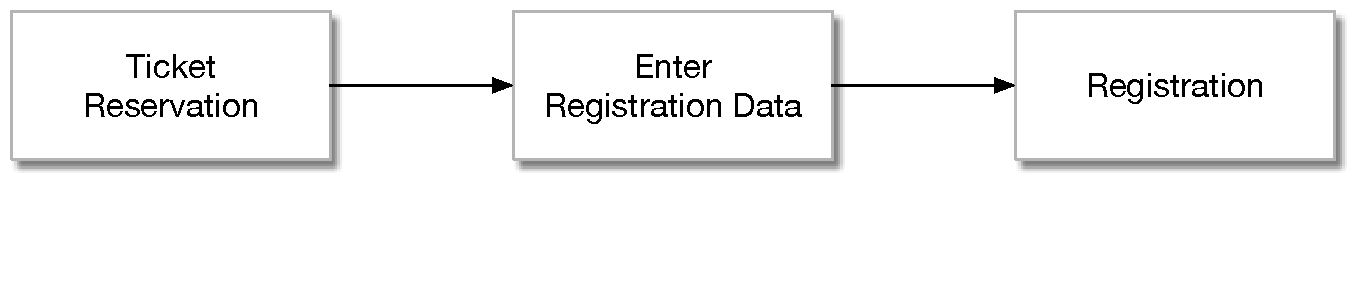
\includegraphics[width=\textwidth]{../Registration3.pdf}
\end{onlyenv}

\begin{onlyenv}<5>
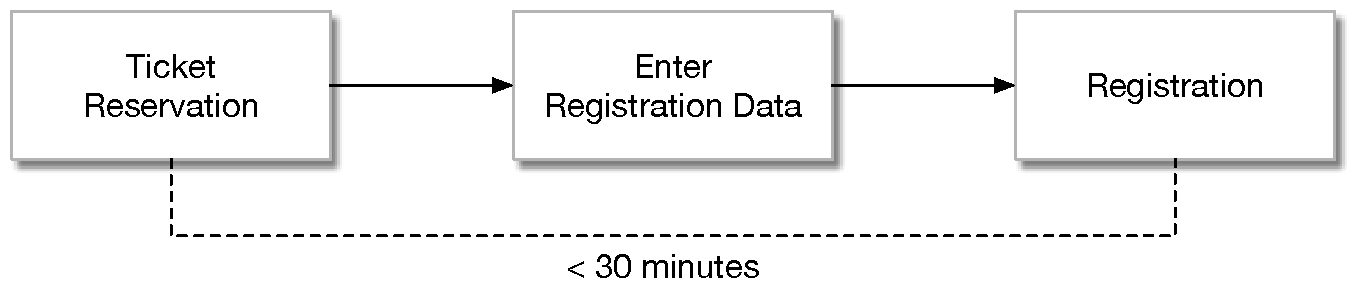
\includegraphics[width=\textwidth]{../Registration4.pdf}
\end{onlyenv}

\end{frame}

%%%%%%%%%%%%%%%%%%%%%%%%%%%%%%%%%%%%%%%%%%%%%%%%%%
\begin{frame}[fragile]{}

\renewcommand{\SPACE}{1em}

11 users encountered this bug:

\vspace{\SPACE}                 

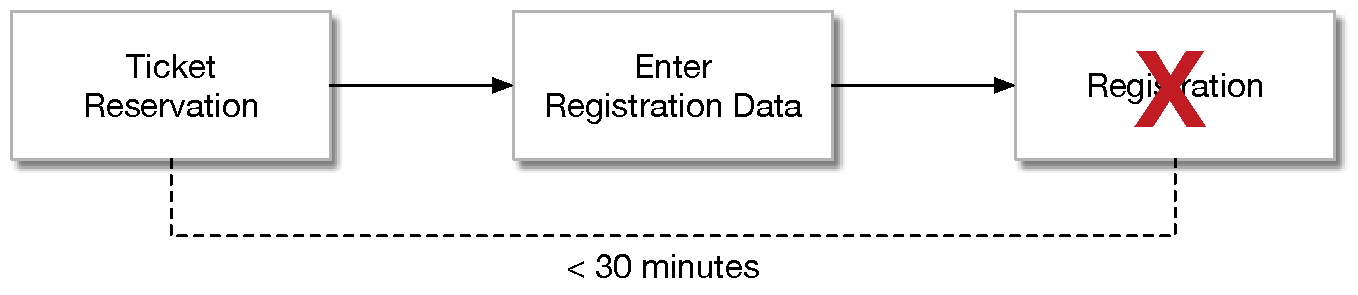
\includegraphics[width=\textwidth]{../Registration5.pdf}

\vspace{\SPACE}                 

\onslide+<2->


\includegraphics[width=\textwidth]{../subscription_problem.png}

\onslide+<3->
                  
\vspace{\SPACE}                 
                  
\begin{itemize}
\item only 2 or 3 users complained
\item reservation token only contained session id
\item was deleted after 30 minutes
\end{itemize}
                  
$\Longrightarrow$ who actually made the reservation?
             
\end{frame}

%%%%%%%%%%%%%%%%%%%%%%%%%%%%%%%%%%%%%%%%%%%%%%%%%%
\begin{frame}[fragile]{}

\begin{center}
\LARGE
How can this be improved?
\end{center}             
                  
\end{frame}

%%%%%%%%%%%%%%%%%%%%%%%%%%%%%%%%%%%%%%%%%%%%%%%%%%
\begin{frame}[fragile]{}

\begin{center}
{
\LARGE
Event Sourcing
}

\vspace{2em}

or:

\vspace{2em}

{
\Large
Don't Drop Data!
}
\end{center}
\end{frame}

%%%%%%%%%%%%%%%%%%%%%%%%%%%%%%%%%%%%%%%%%%%%%%%%%%
\begin{frame}[fragile]{The Classical Approach: Relational Database}

\begin{itemize}                
\item Only captures current state!
\item No information about previous states
\item No information why some change happened
\end{itemize}
                   
\end{frame}

%%%%%%%%%%%%%%%%%%%%%%%%%%%%%%%%%%%%%%%%%%%%%%%%%%
\begin{frame}[fragile]{Idea behind Event Sourcing}

\begin{enumerate}
\item Record all events that happened, and why.
\item Derive the current application state from the recorded events.
\end{enumerate}         



\end{frame}

%%%%%%%%%%%%%%%%%%%%%%%%%%%%%%%%%%%%%%%%%%%%%%%%%%
\begin{frame}[fragile]{Event Sourcing}

\renewcommand{\WIDTH}{.7\textwidth}

\begin{onlyenv}<1>
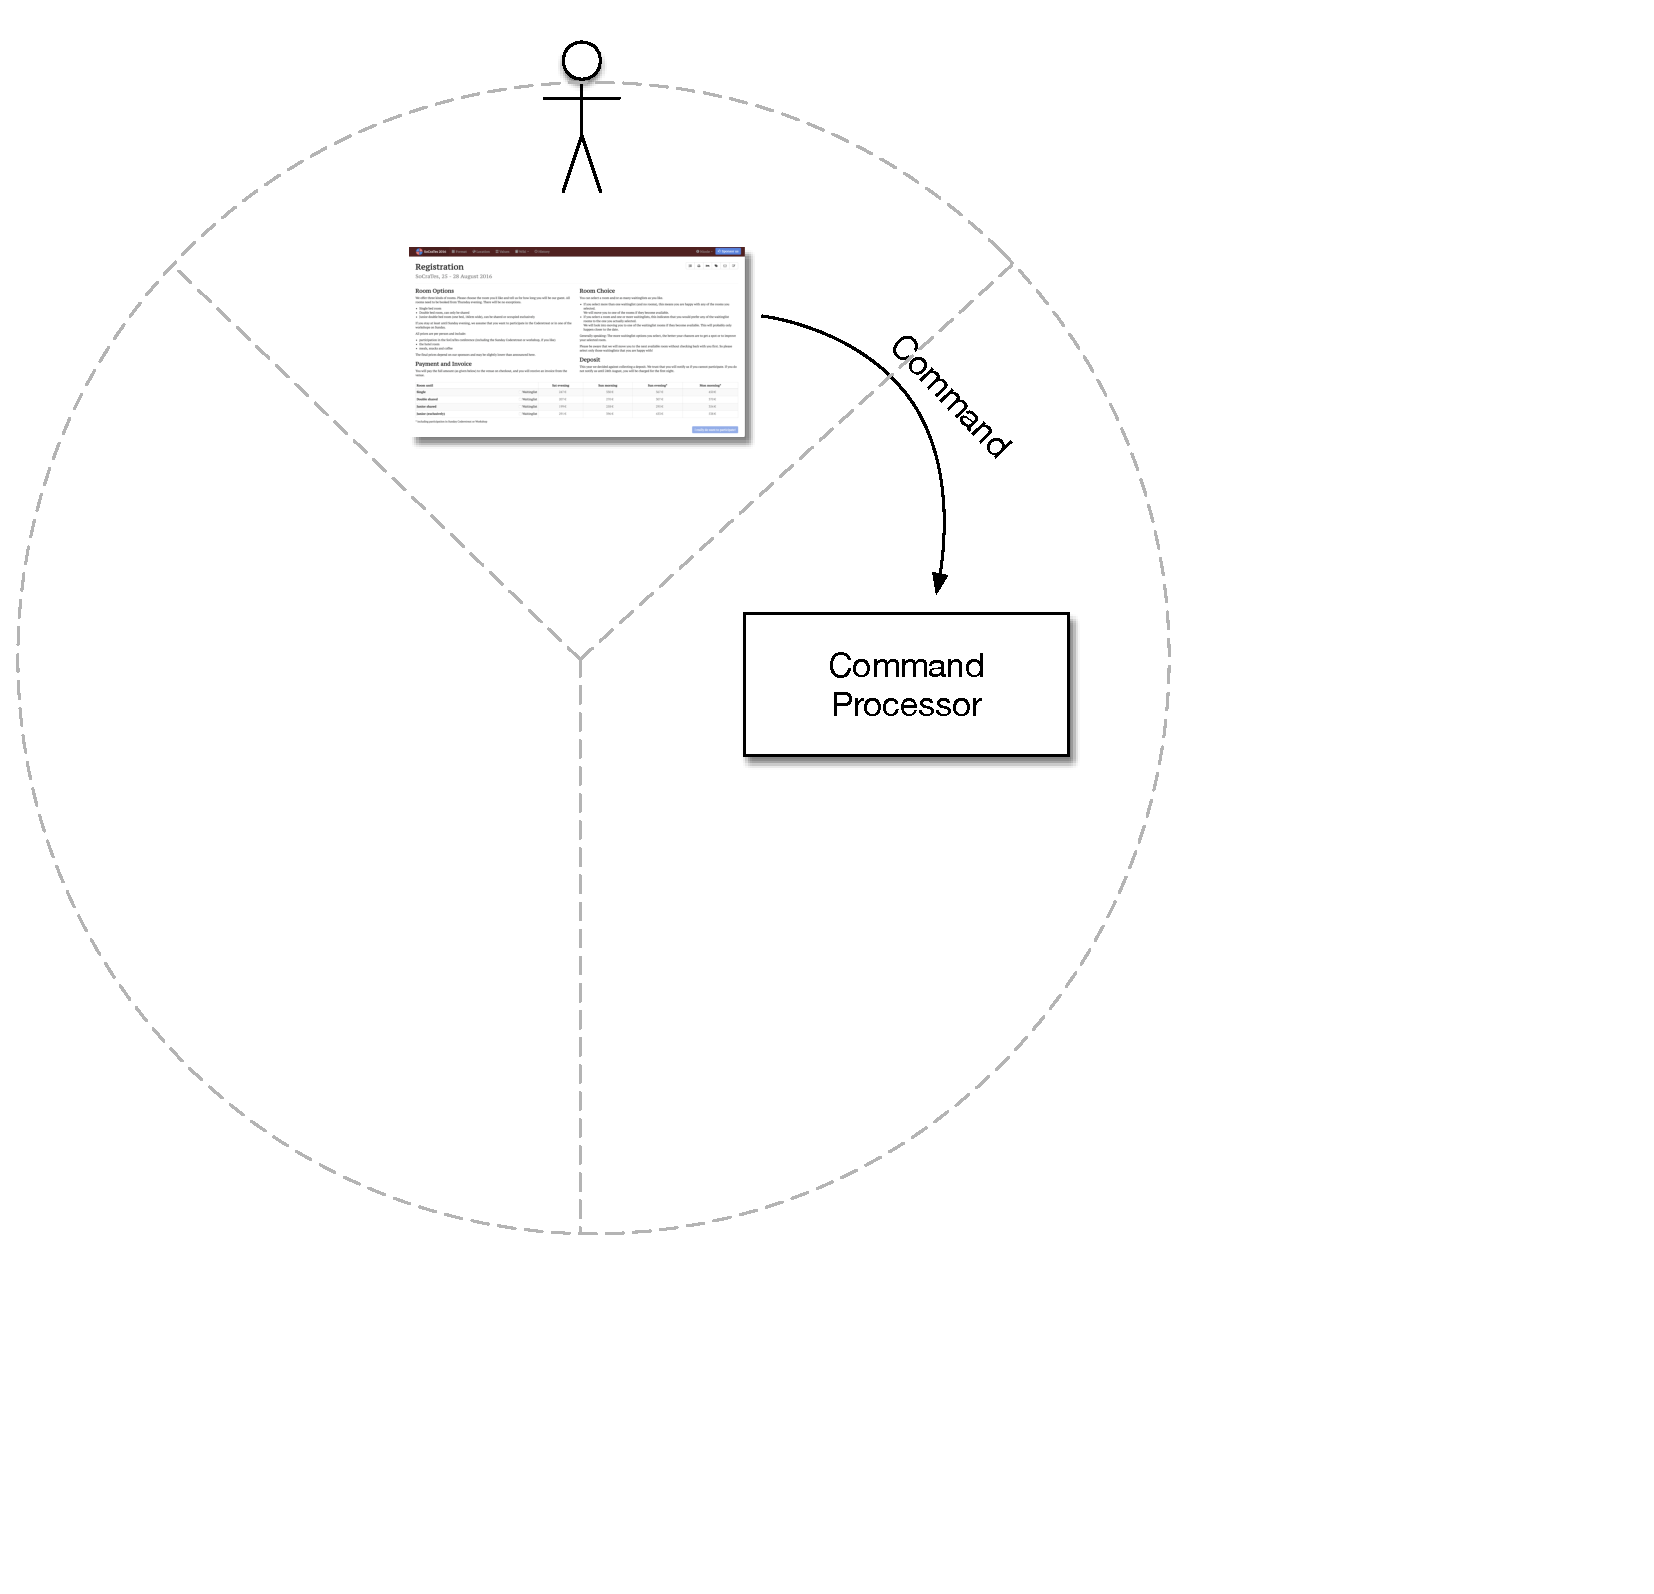
\includegraphics[width=\WIDTH]{../EventSourcing1.pdf} %% command processor
\end{onlyenv}
\begin{onlyenv}<2>
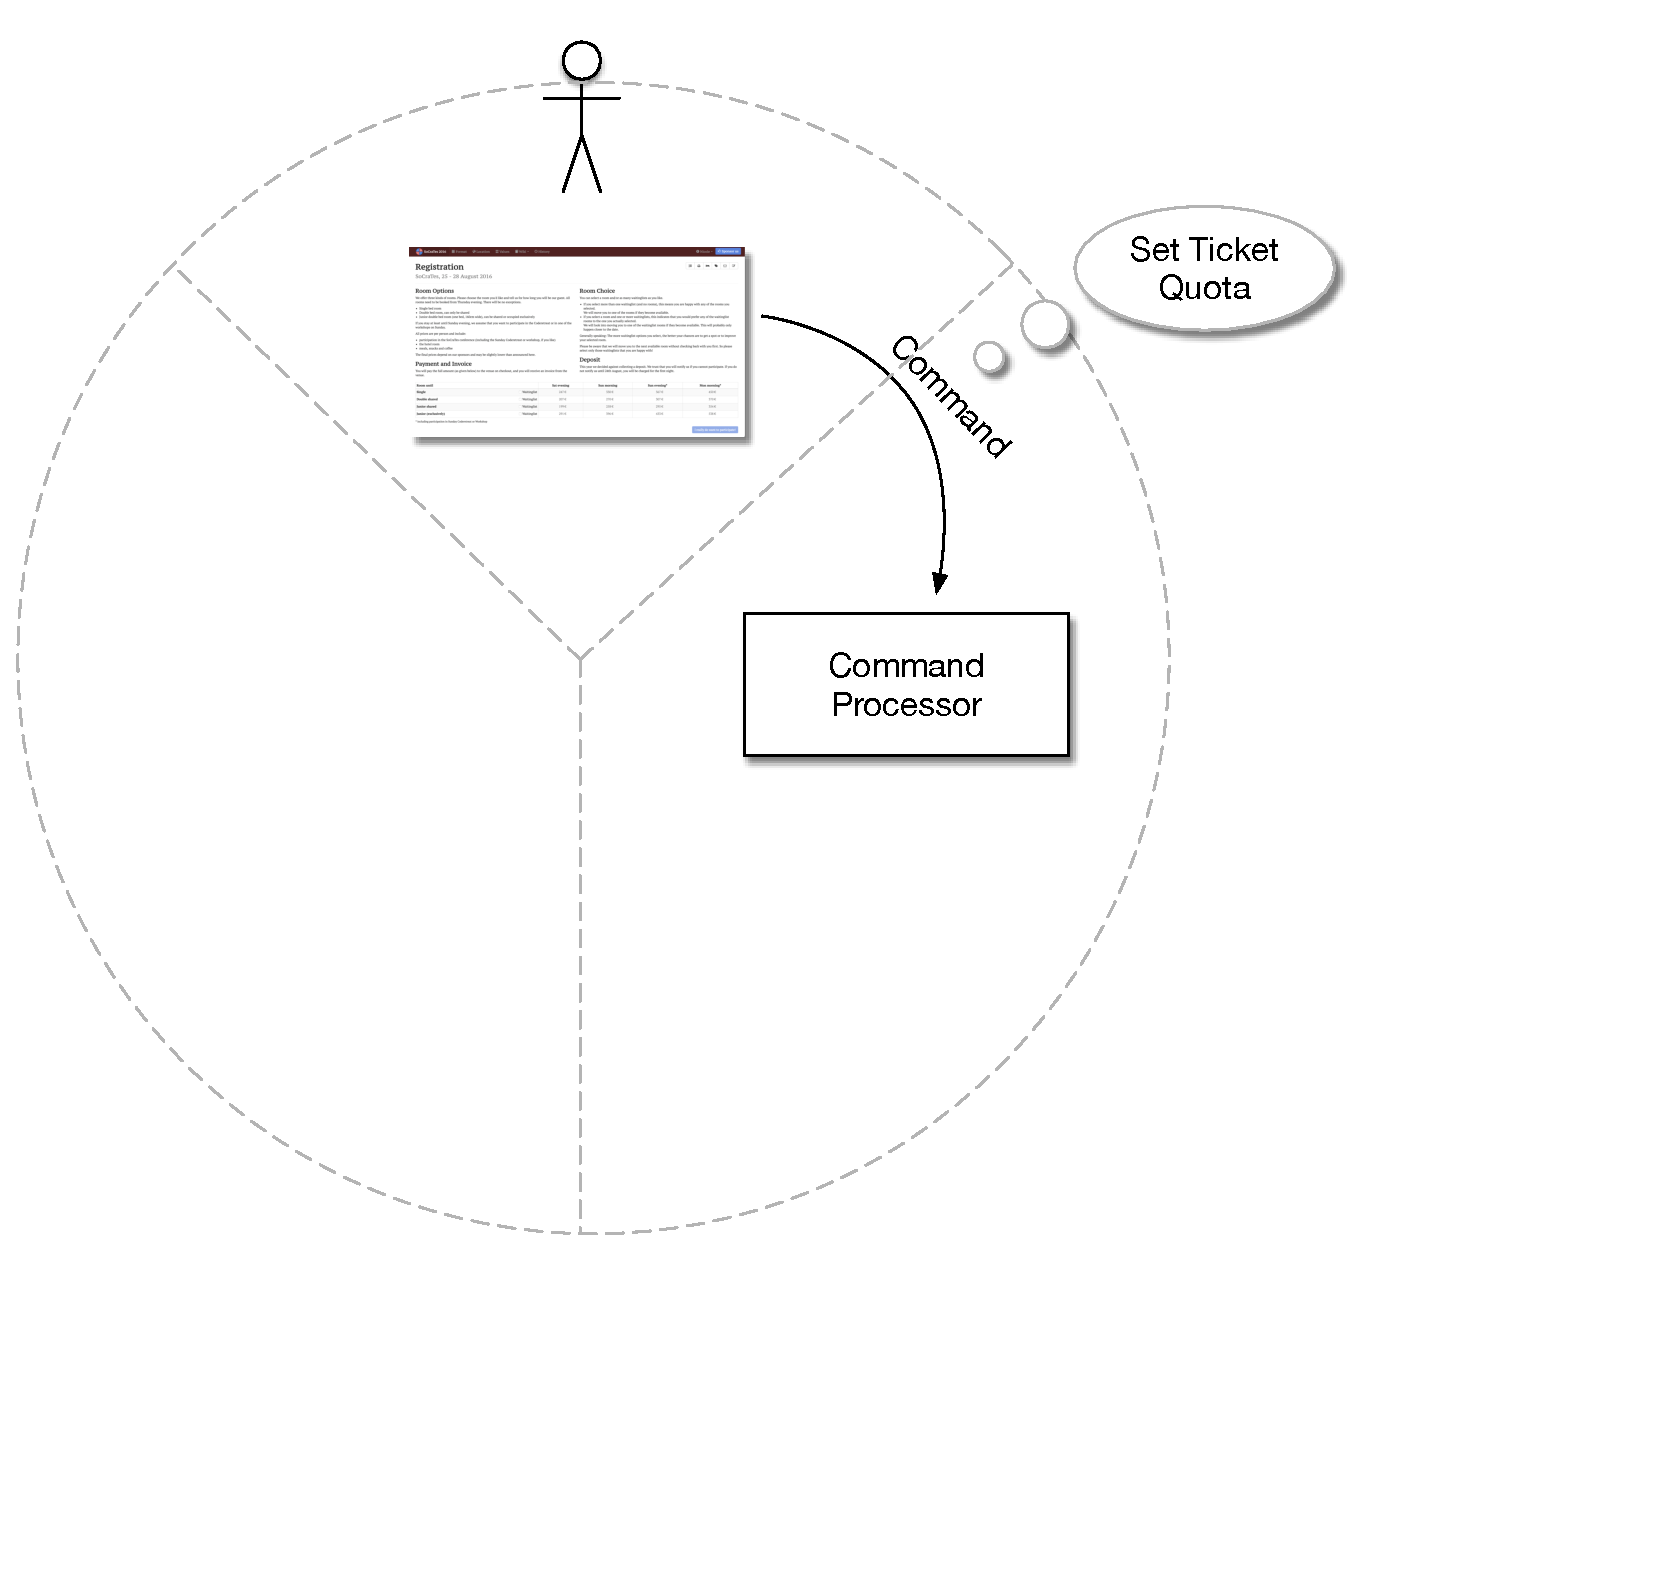
\includegraphics[width=\WIDTH]{../EventSourcing1_1.pdf} %% set ticket quota
\end{onlyenv}
\begin{onlyenv}<3>
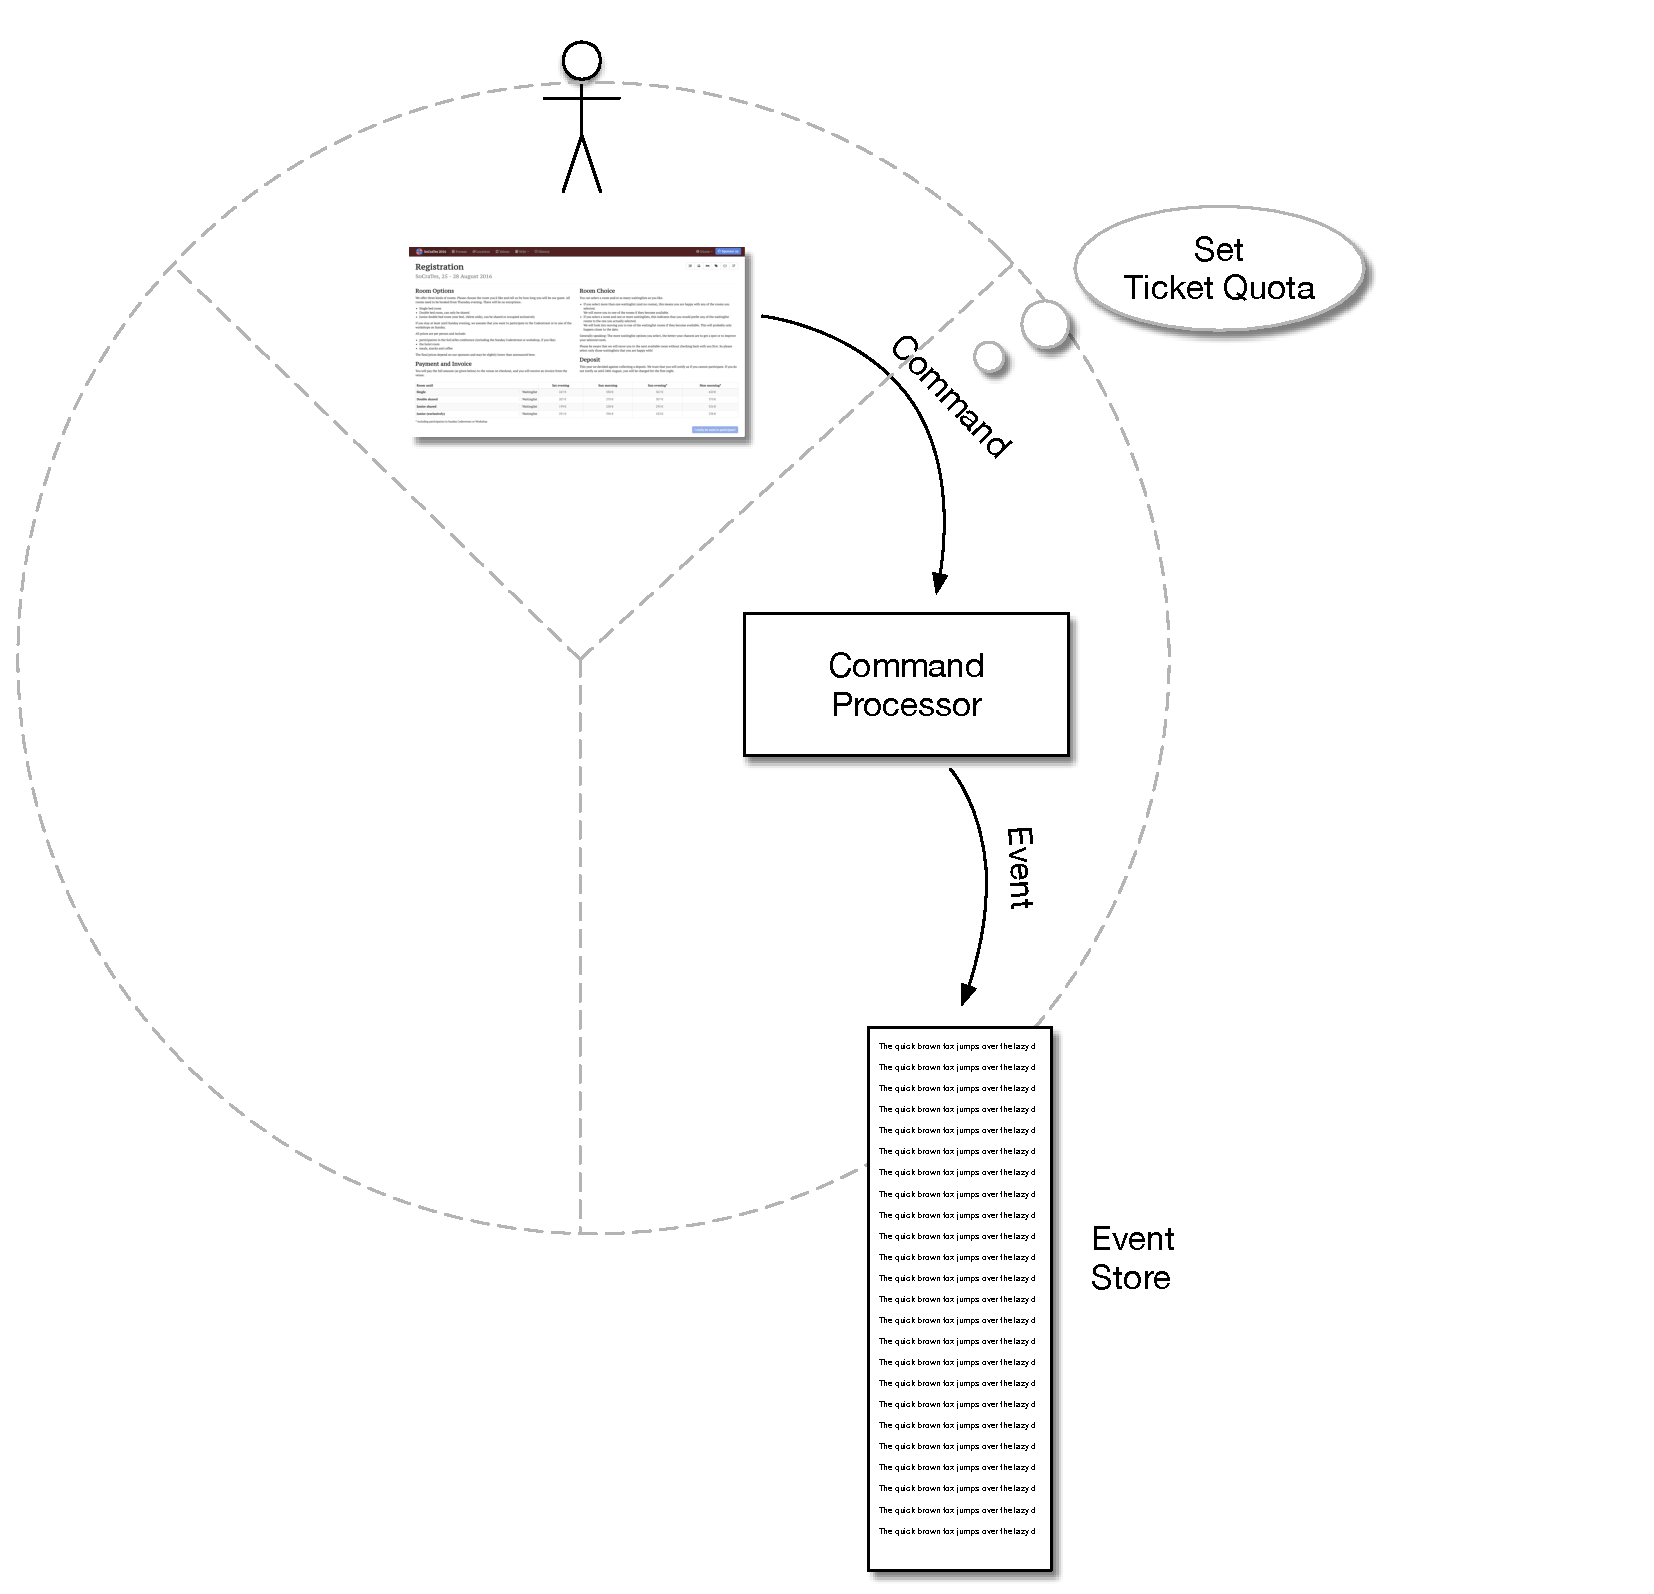
\includegraphics[width=\WIDTH]{../EventSourcing2.pdf} %% event store
\end{onlyenv}
\begin{onlyenv}<4>
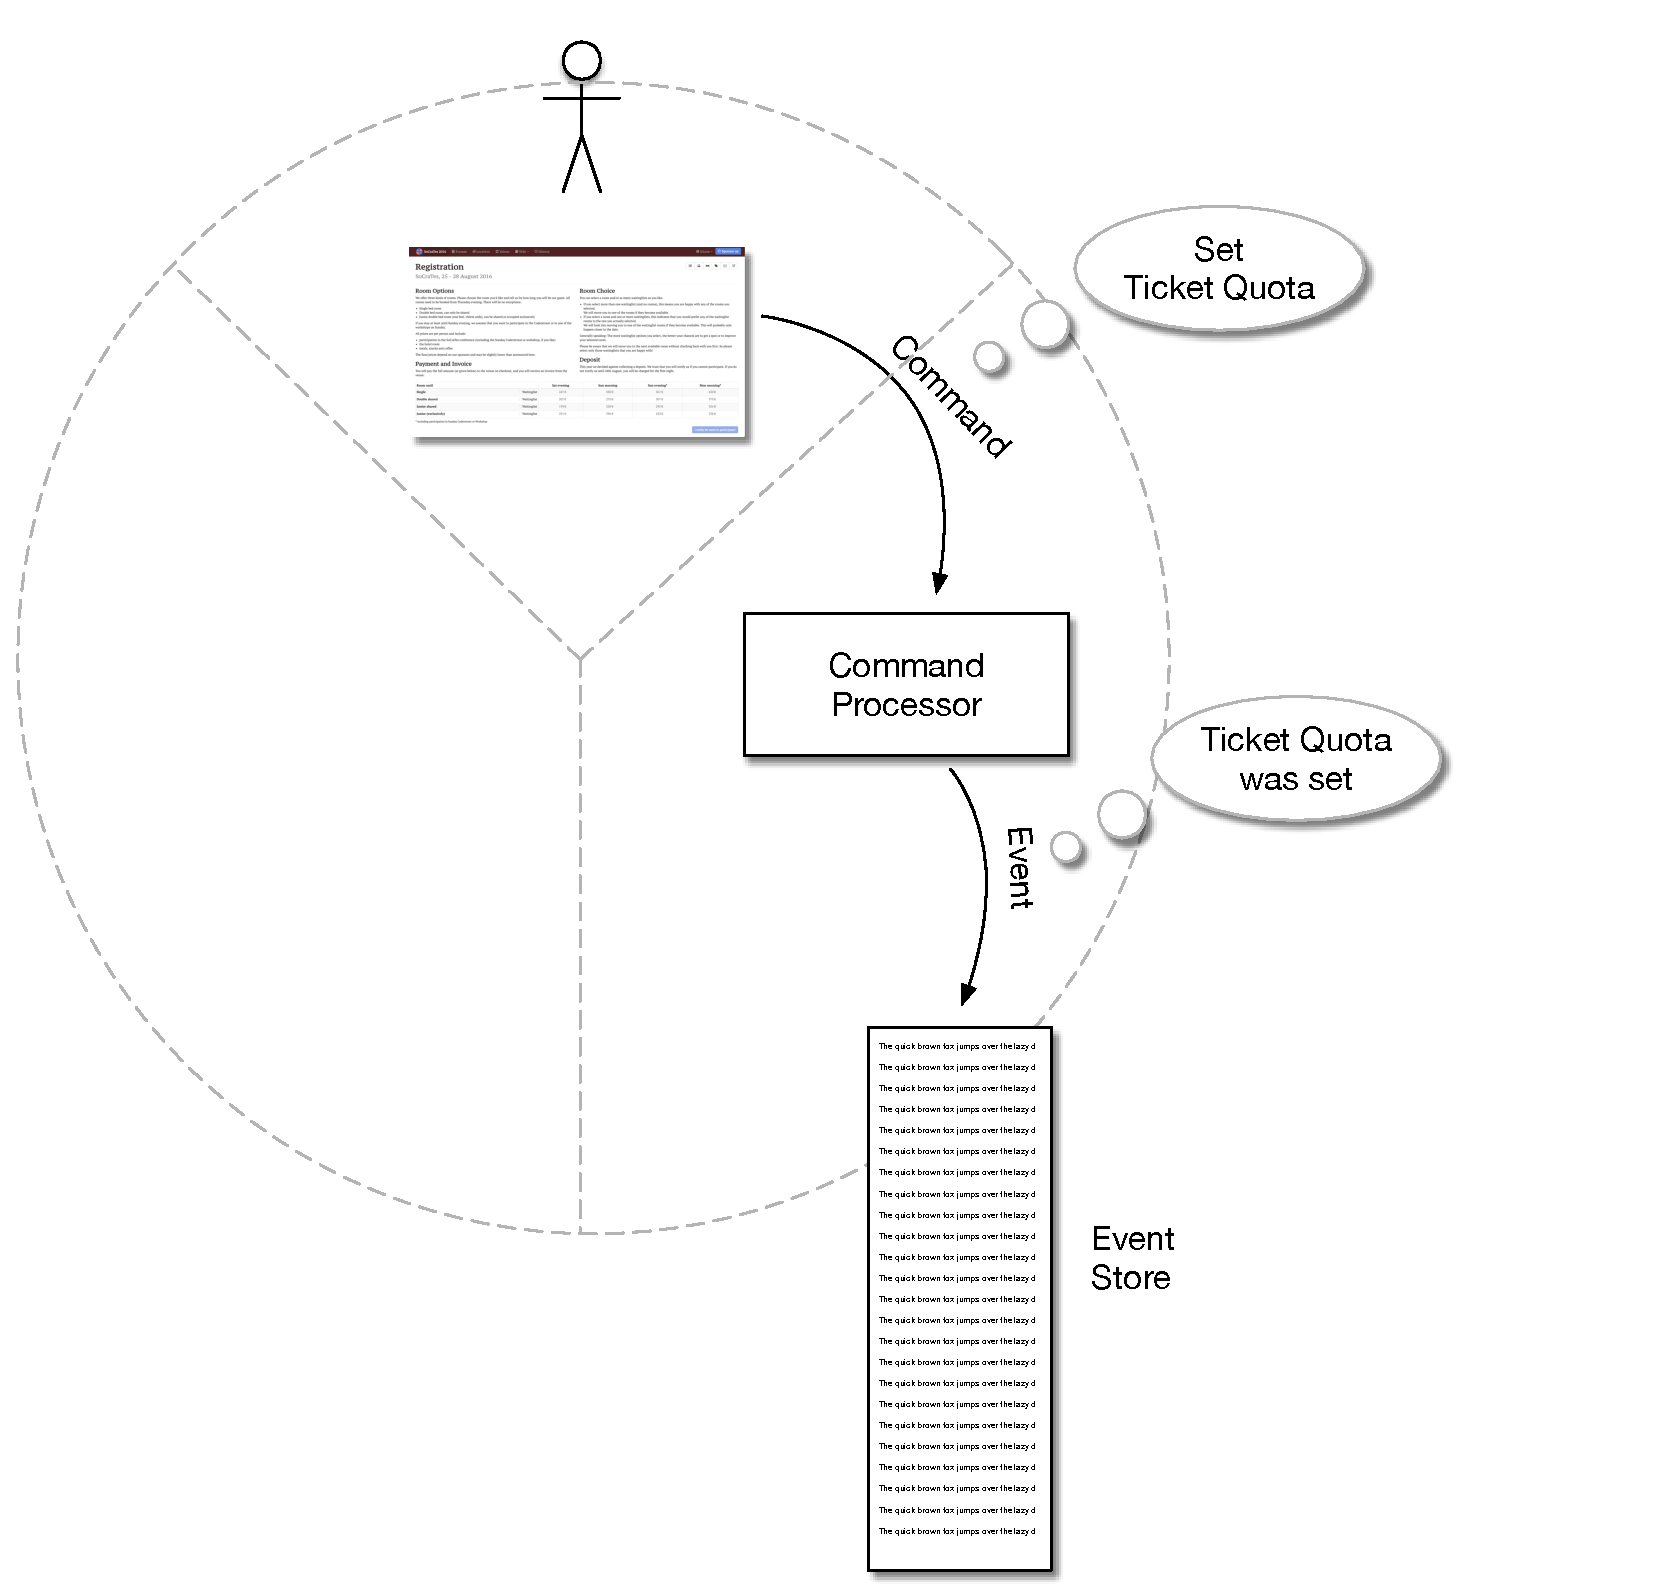
\includegraphics[width=\WIDTH]{../EventSourcing2_1.pdf} %% ticket quota was set
\end{onlyenv}
\begin{onlyenv}<5>
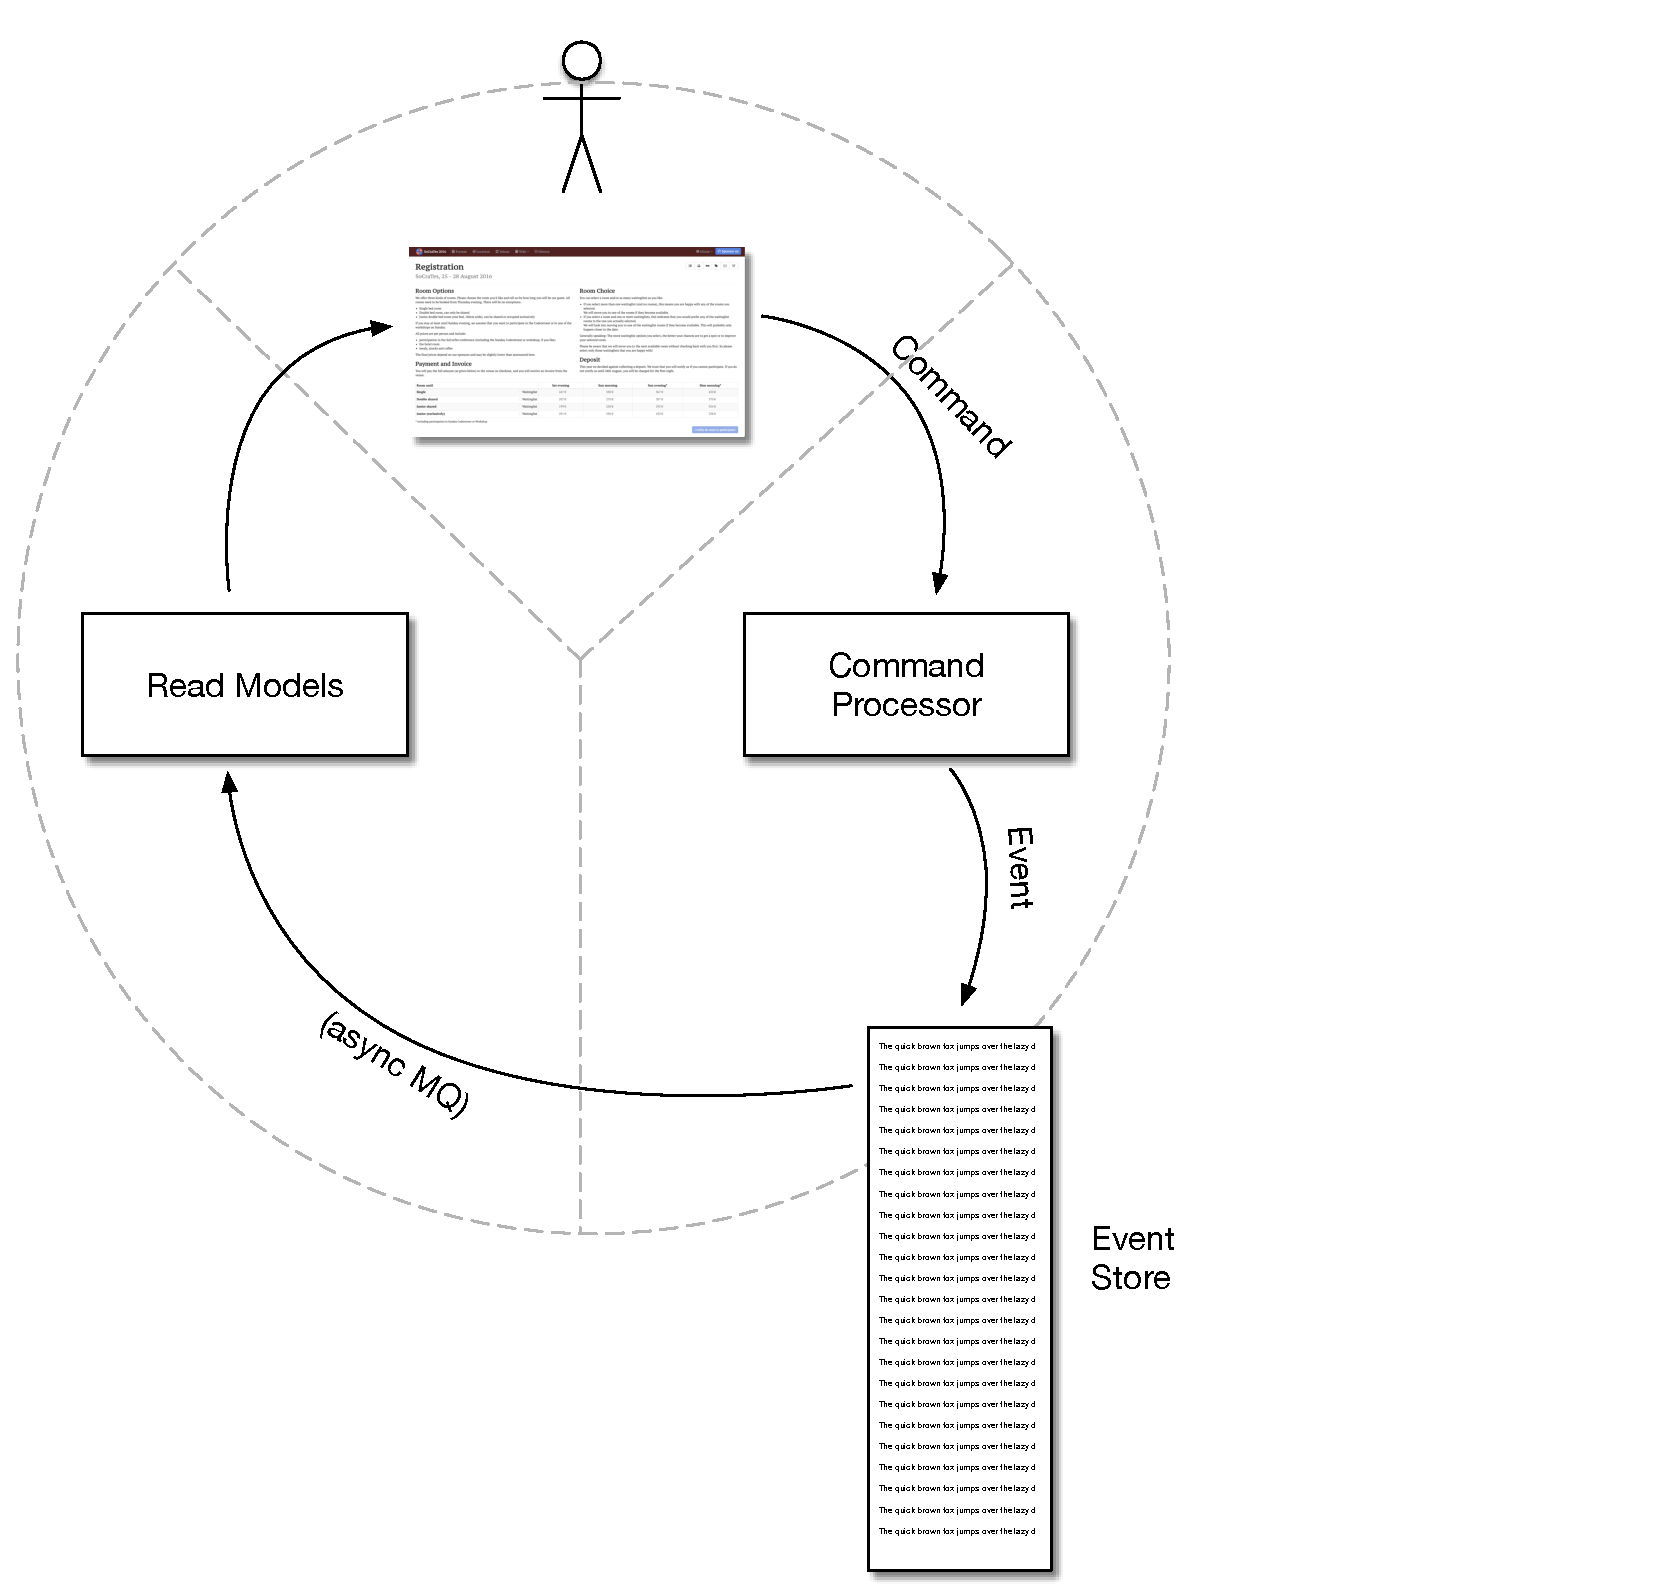
\includegraphics[width=\WIDTH]{../EventSourcing3.pdf} %% read models
\end{onlyenv}
\begin{onlyenv}<6>
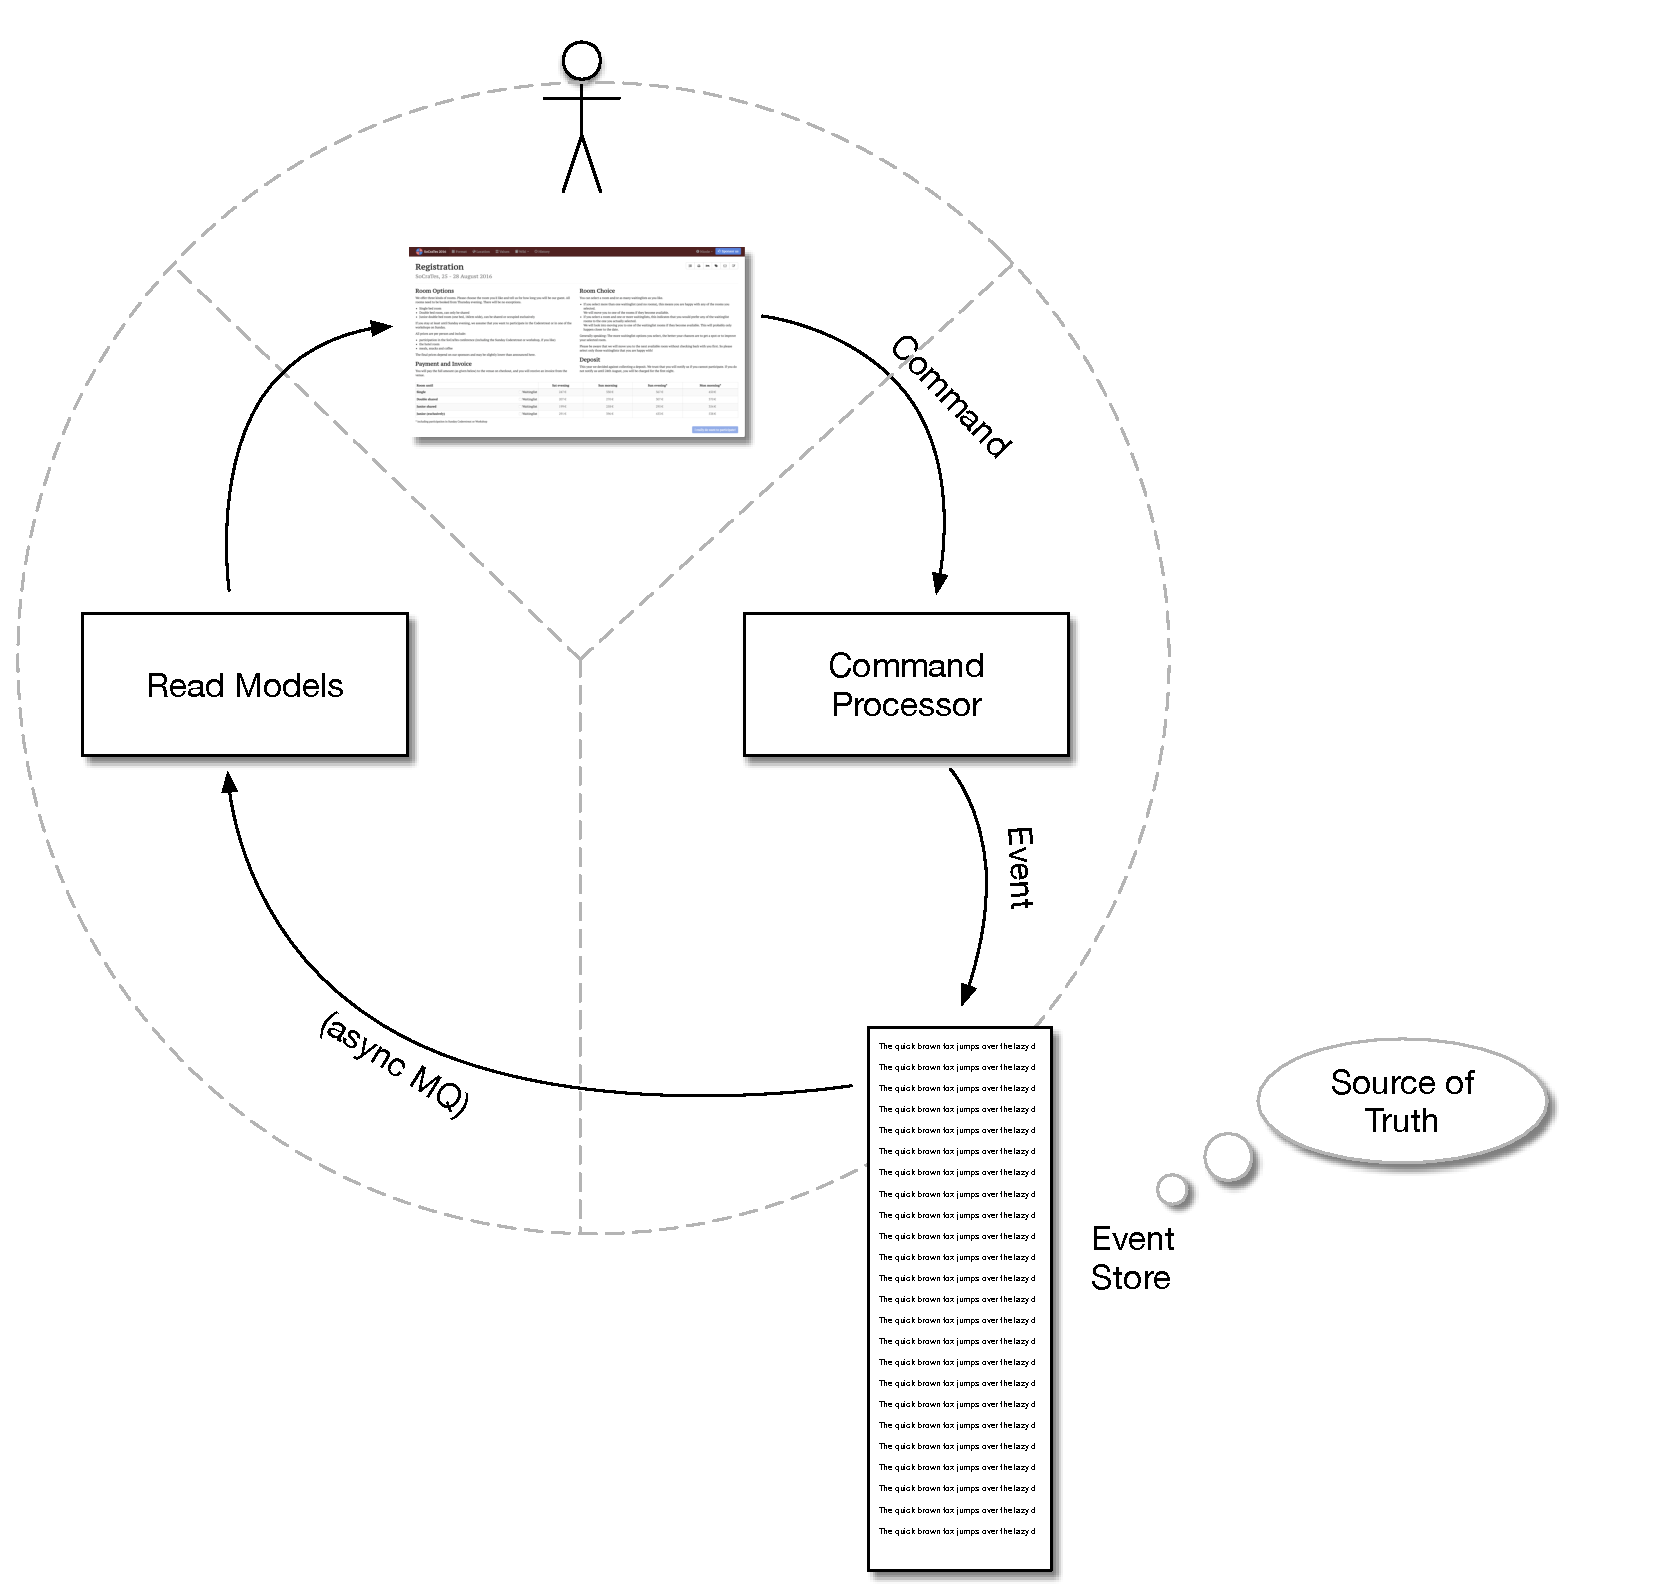
\includegraphics[width=\WIDTH]{../EventSourcing3_0.pdf} %% source of truth
\end{onlyenv}
\begin{onlyenv}<7>
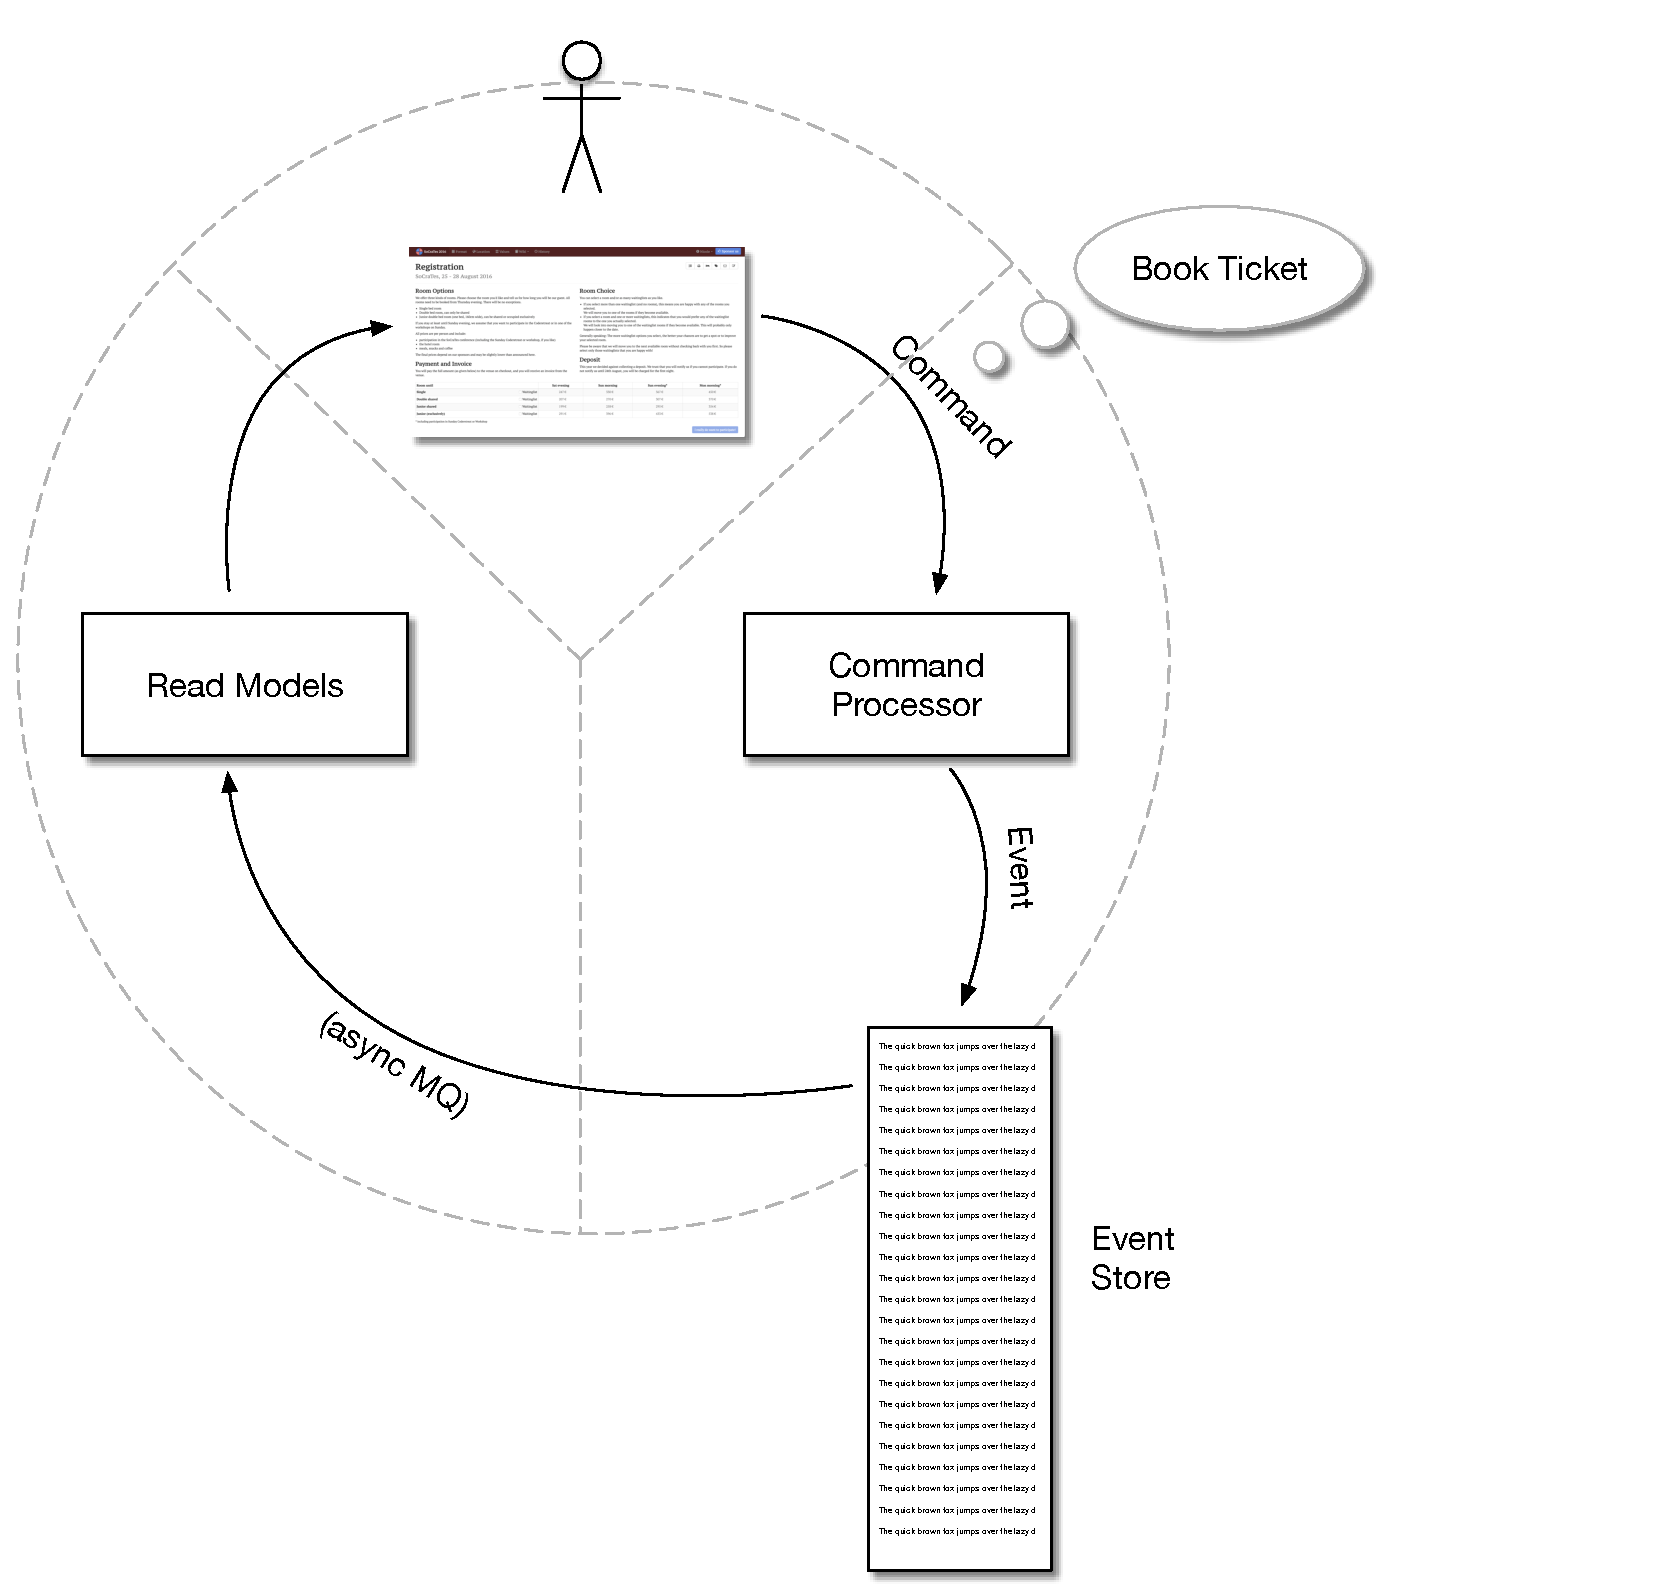
\includegraphics[width=\WIDTH]{../EventSourcing3_1.pdf} %% book ticket
\end{onlyenv}
\begin{onlyenv}<8>
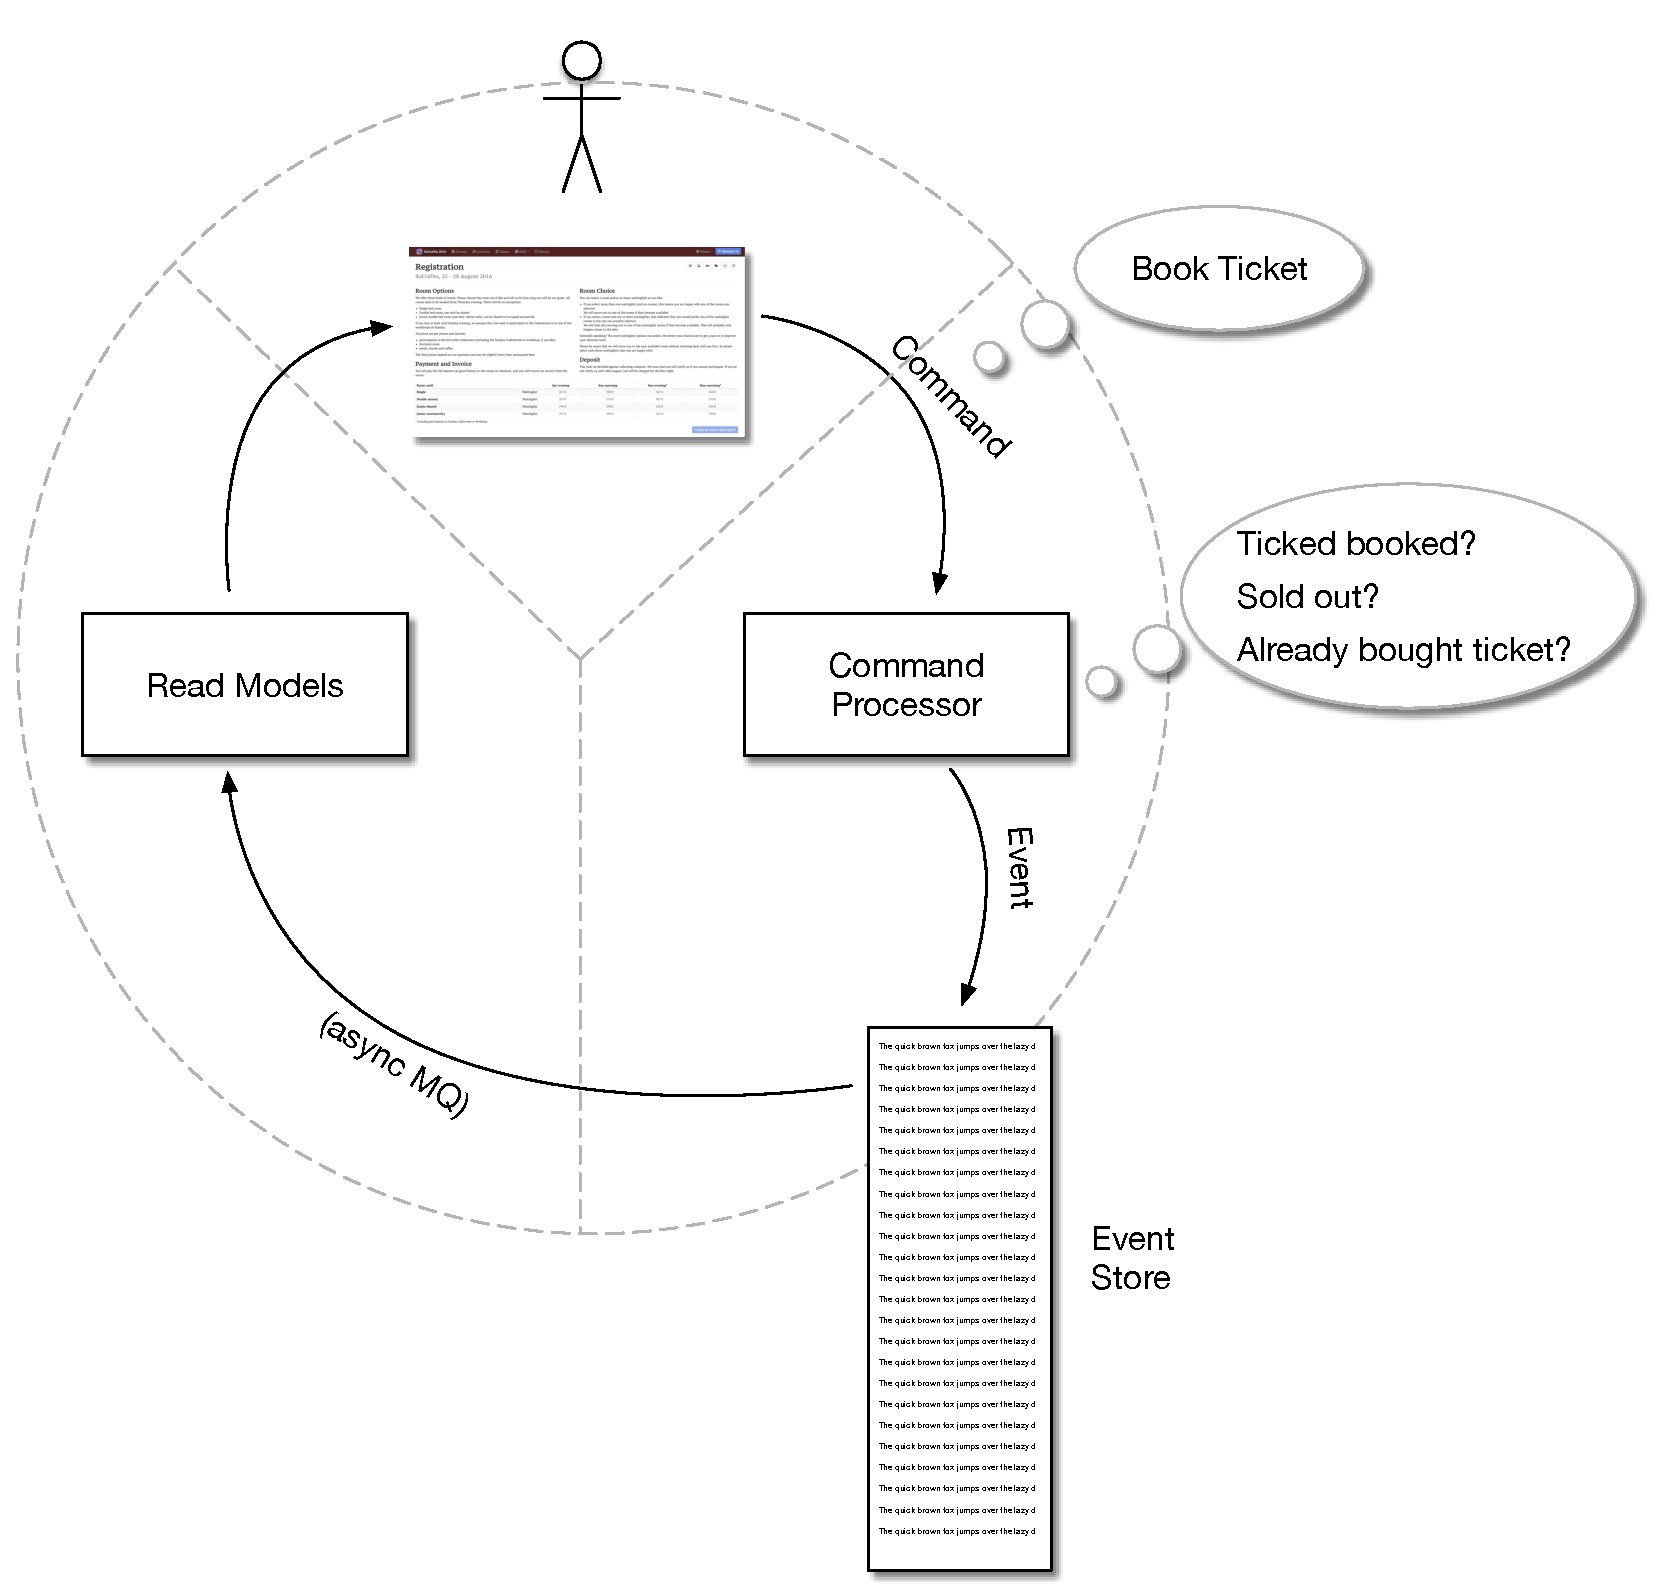
\includegraphics[width=\WIDTH]{../EventSourcing3_2.pdf} %% which event to reply?
\end{onlyenv}
\begin{onlyenv}<9>
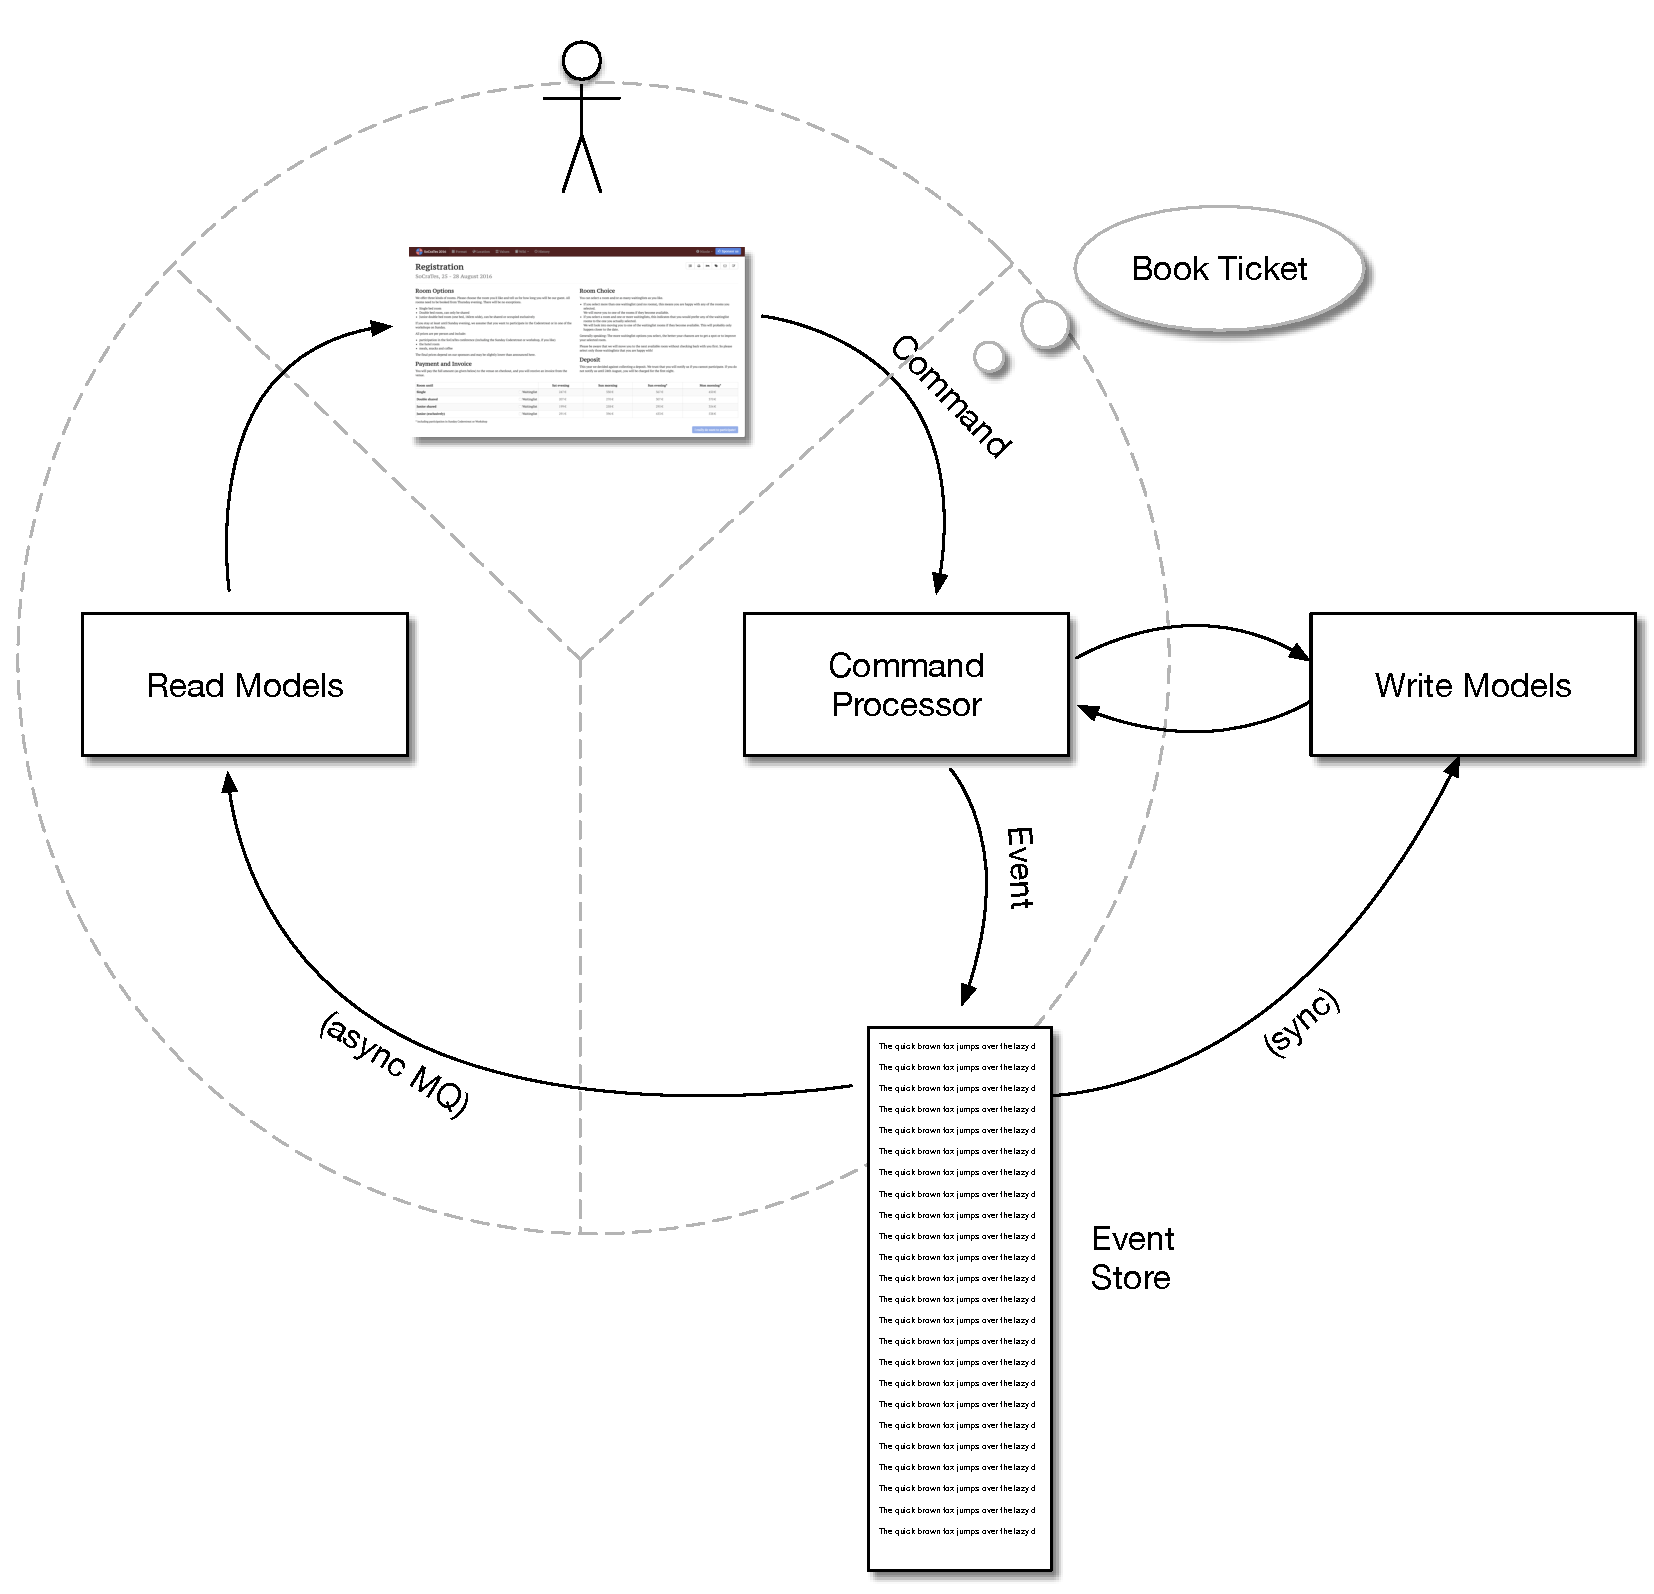
\includegraphics[width=\WIDTH]{../EventSourcing4.pdf} %% write models
\end{onlyenv}
\begin{onlyenv}<10>
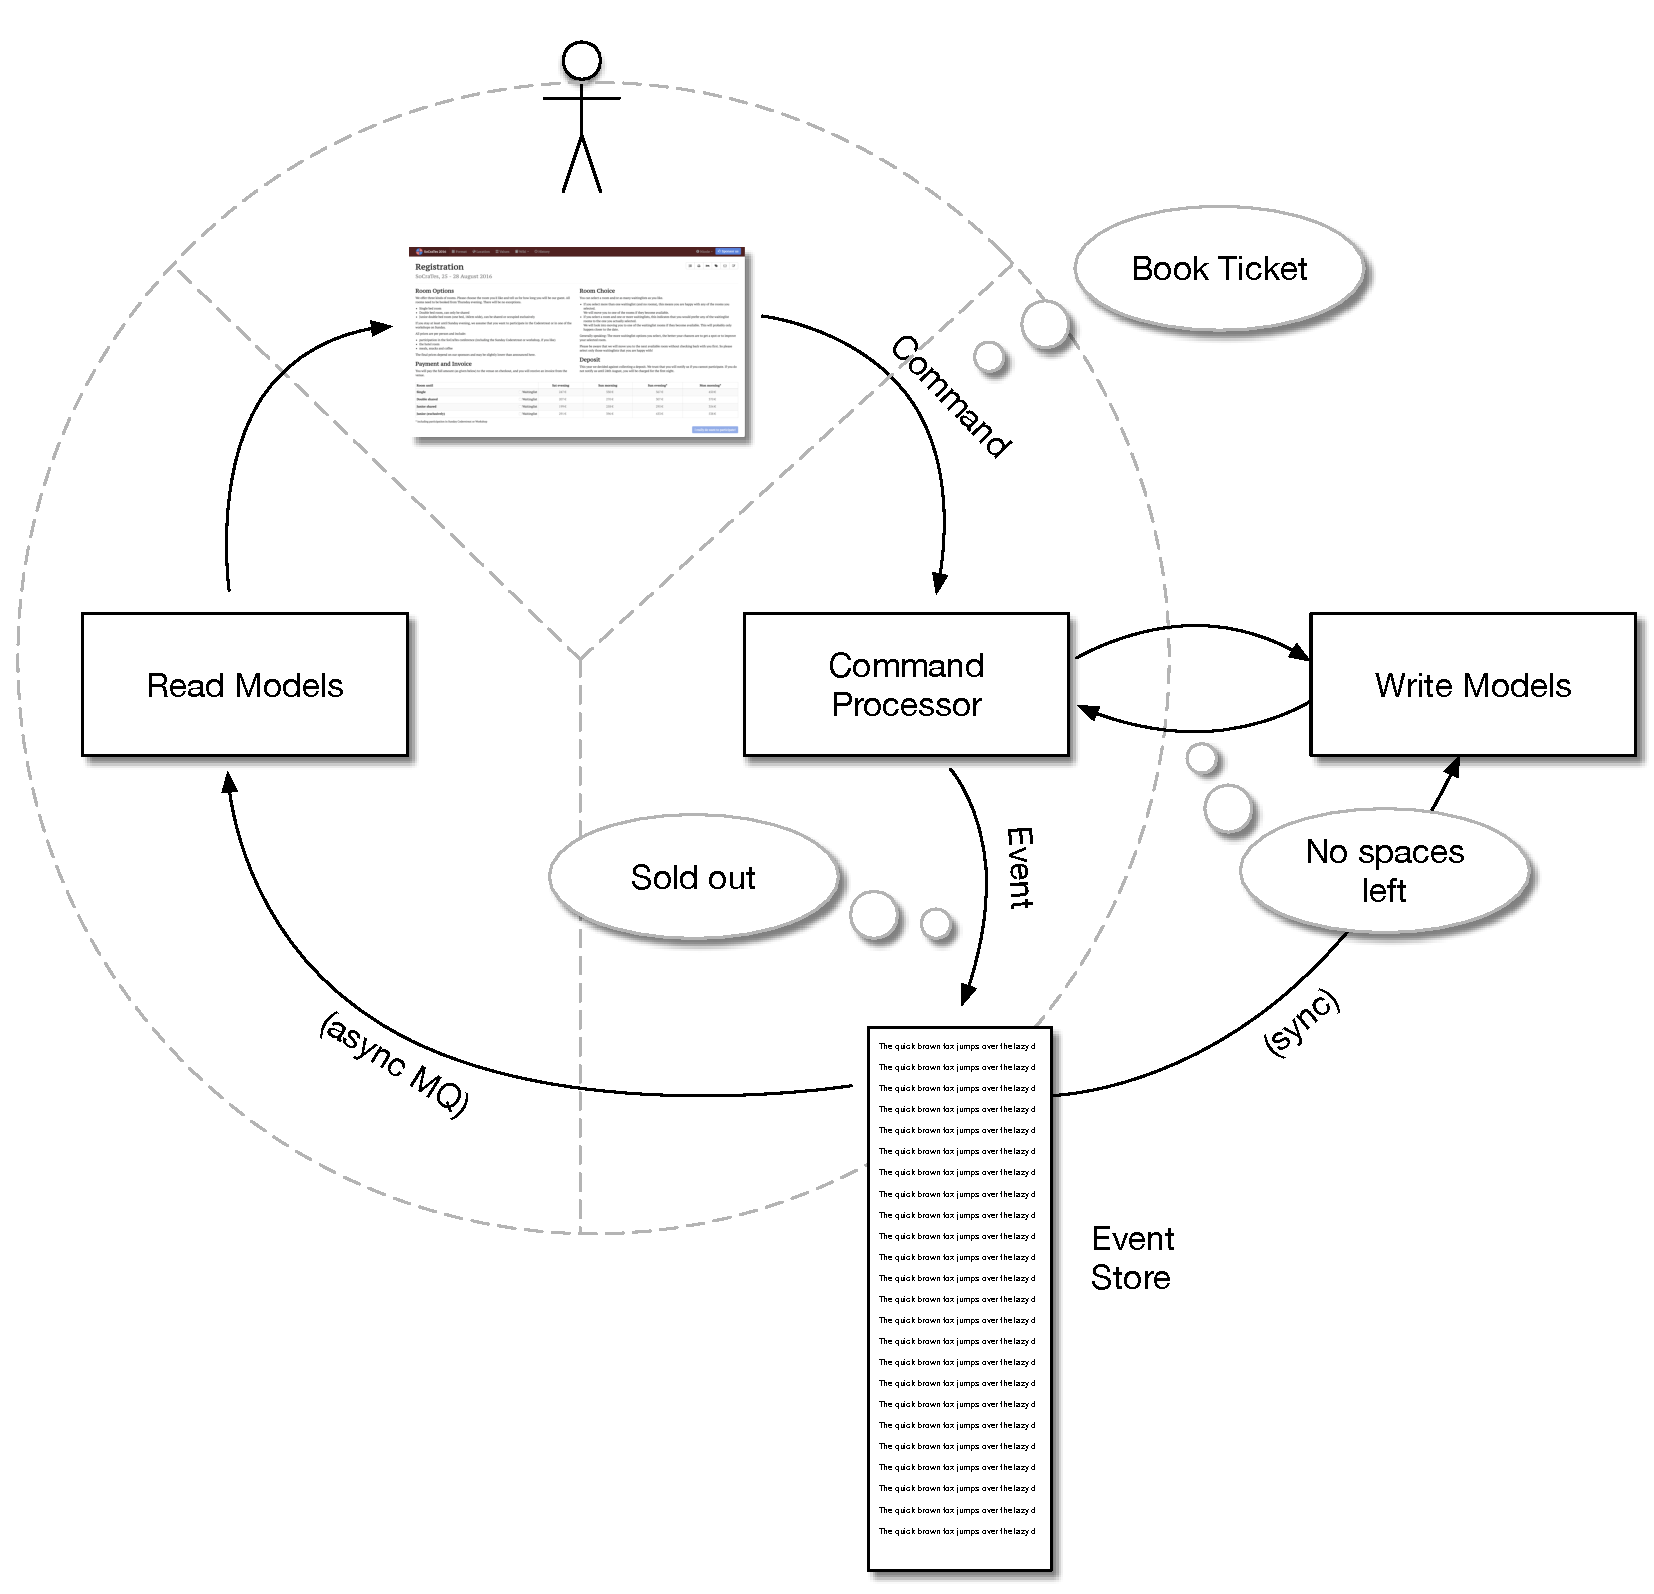
\includegraphics[width=\WIDTH]{../EventSourcing5.pdf} %% sold out
\end{onlyenv}

\end{frame}

%%%%%%%%%%%%%%%%%%%%%%%%%%%%%%%%%%%%%%%%%%%%%%%%%%
\begin{frame}[fragile]{Standard Event Sourcing Scenario}

\begin{itemize}
\item Event sourcing in application server
\item Incremental updates of event store, write models and read models
\item Write models must be updated synchronously
\item Read models can be updated asynchronously
\end{itemize}

\end{frame}

%%%%%%%%%%%%%%%%%%%%%%%%%%%%%%%%%%%%%%%%%%%%%%%%%%
\begin{frame}[fragile]{Our Decision}

\begin{itemize}
\item Experiment with Event Sourcing
\item Only for registration
\item Constraint: No overbookings!
\end{itemize}

\end{frame}


%%%%%%%%%%%%%%%%%%%%%%%%%%%%%%%%%%%%%%%%%%%%%%%%%%
\begin{frame}[fragile]{The Ticket Quota}

\begin{onlyenv}<1-3>
The event constants:

\begin{highlight}{1}
module.exports = {
  TICKET_QUOTA_WAS_SET: 'TICKET-QUOTA-WAS-SET',
  // ...
}
\end{highlight}

\onslide+<2->
The event constructor:

\begin{highlight}{2}
ticketQuotaWasSet: function (quota) {
    return {event: e.TICKET_QUOTA_WAS_SET, quota};
}
\end{highlight}

\onslide+<3->
\begin{highlight}{3}
CommandProcessor.prototype.setQuota = function (newQuota) {
  return roomQuotaWasSet(newQuota);
};
\end{highlight}
\end{onlyenv}

\begin{onlyenv}<4->
\begin{highlight}{4}
function ReadModel(events) {
  this._quota = undefined;
  this.process(events);
}
\end{highlight}
\onslide+<5->
\begin{highlight}{5}
ReadModel.prototype.process = function (events) {
  this._quota = R.reduce(processQuota, this._quota, events);
};
\end{highlight}
\onslide+<6->
\begin{highlight}{6}
var processQuota = function (quota, event) {
  return event.event === e.ROOM_QUOTA_WAS_SET ? event.quota : quota;
};
\end{highlight}
\onslide+<7->
\begin{highlight}{7}
ReadModel.prototype.quota = function () {
  return this._quota;
};
\end{highlight}
\end{onlyenv}

\end{frame}

%%%%%%%%%%%%%%%%%%%%%%%%%%%%%%%%%%%%%%%%%%%%%%%%%%
\begin{frame}[fragile]{On Opening the Registration}

\onslide+<2->

Registration began...

\onslide+<3->

\vspace{3em}

~ \hspace{10em} ... but nobody registered!
 
\end{frame}


%%%%%%%%%%%%%%%%%%%%%%%%%%%%%%%%%%%%%%%%%%%%%%%%%%
\begin{frame}[fragile]{}

\begin{center}
\Huge
What happened???
\end{center}

\end{frame}

%%%%%%%%%%%%%%%%%%%%%%%%%%%%%%%%%%%%%%%%%%%%%%%%%%
\begin{frame}[fragile]{Event Sourcing in Node.js}

Let's understand how node.js works

\end{frame}

%%%%%%%%%%%%%%%%%%%%%%%%%%%%%%%%%%%%%%%%%%%%%%%%%%
\begin{frame}[fragile]{Node.js}

\renewcommand{\WIDTH}{\textwidth}

\begin{columns}[T] % align columns
\begin{column}{.7\textwidth}
\begin{onlyenv}<1>
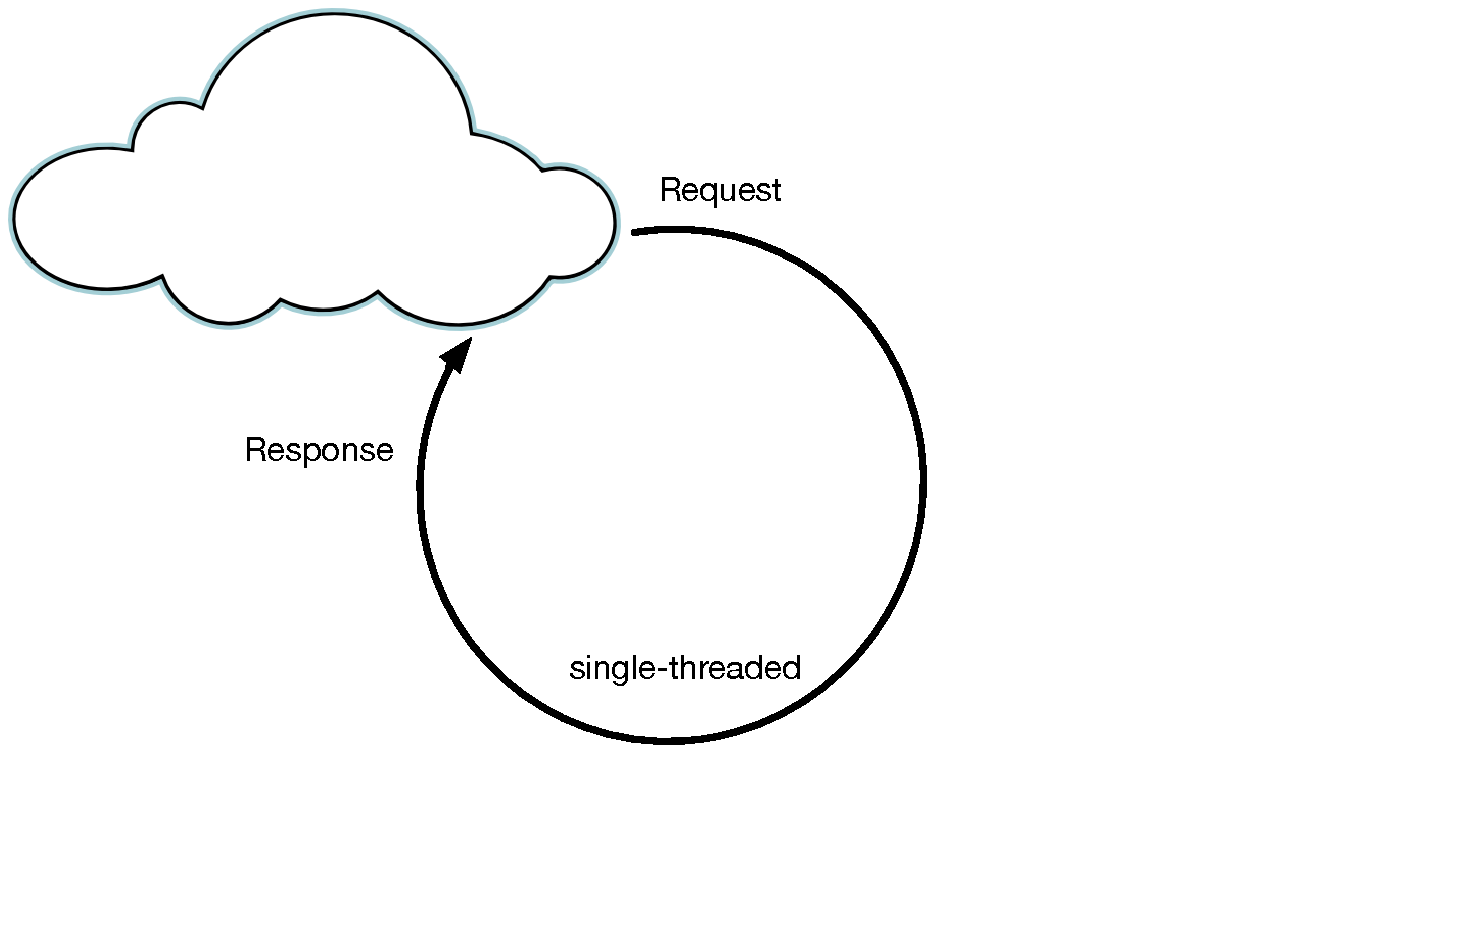
\includegraphics[width=\WIDTH]{../Nodejs1.pdf}
\end{onlyenv}

\begin{onlyenv}<2>
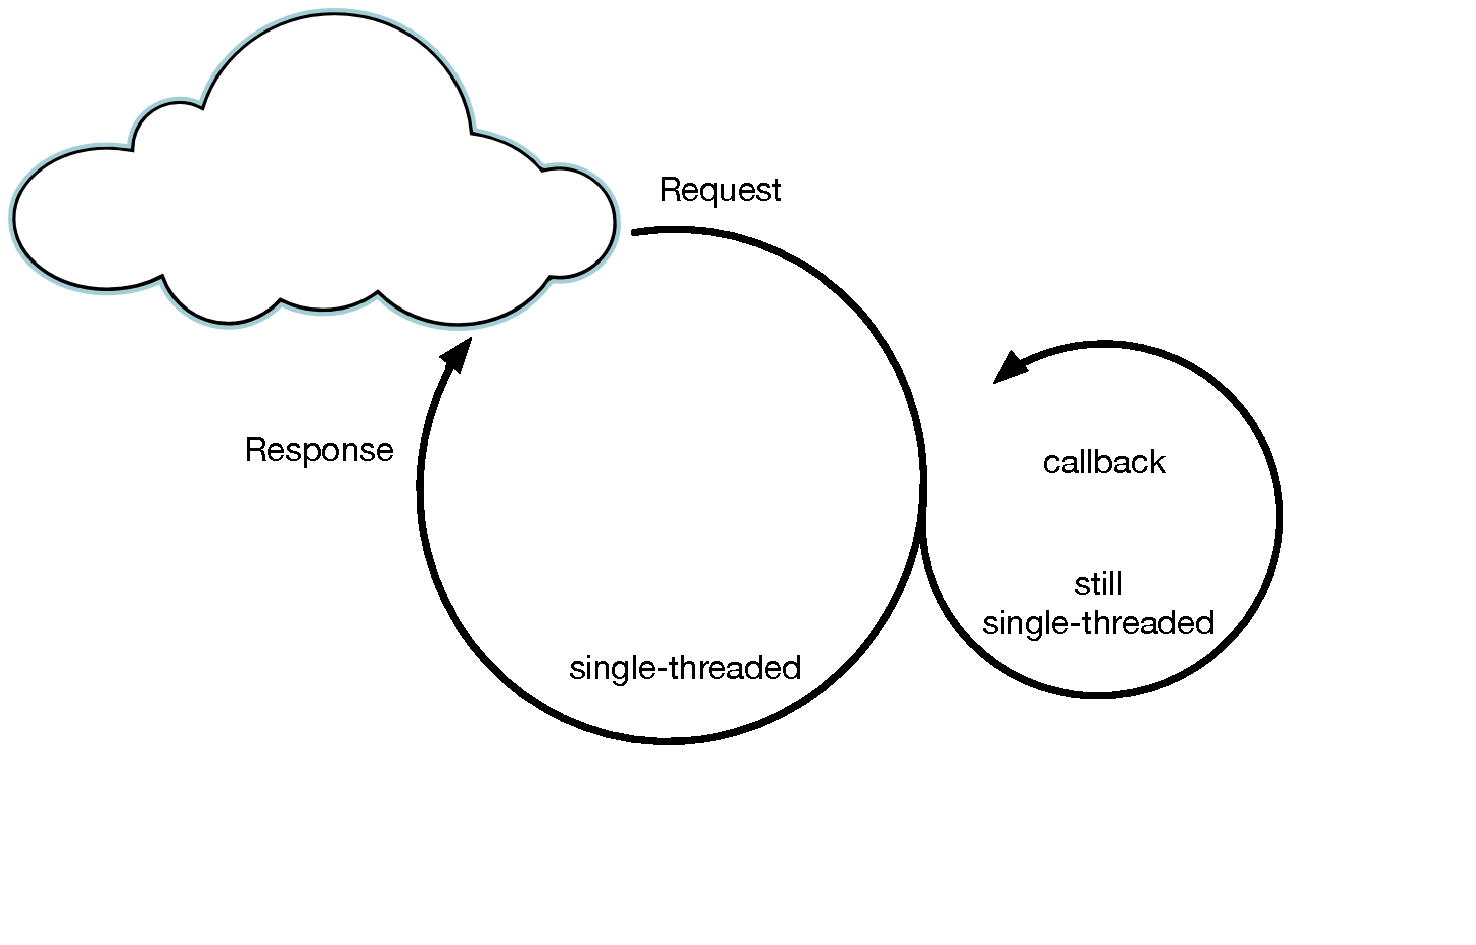
\includegraphics[width=\WIDTH]{../Nodejs2.pdf}
\end{onlyenv}

\begin{onlyenv}<3>
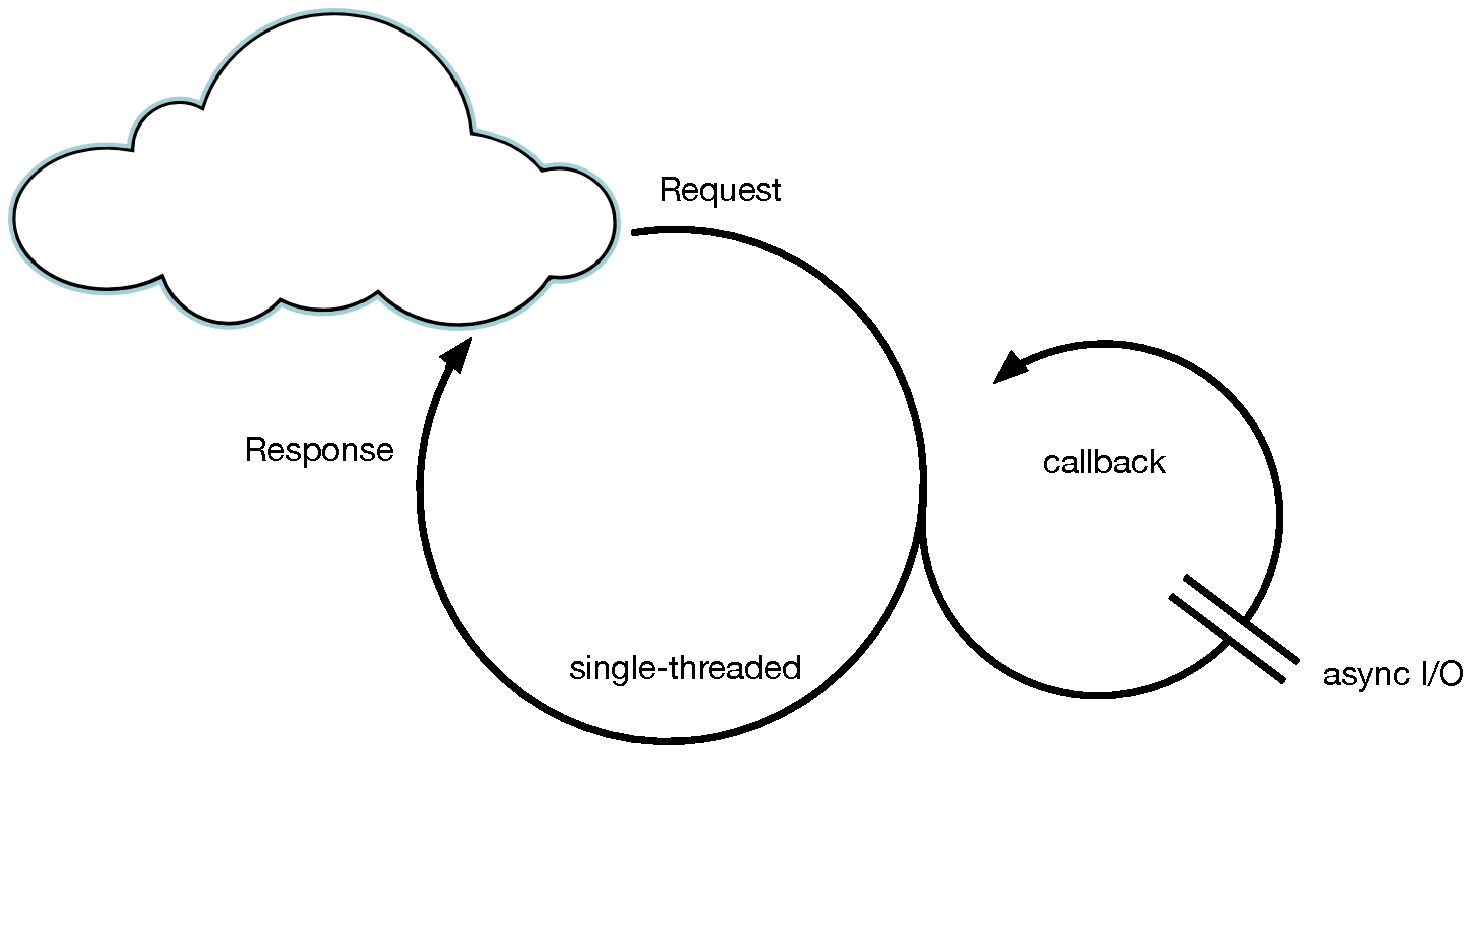
\includegraphics[width=\WIDTH]{../Nodejs3.pdf}
\end{onlyenv}

\begin{onlyenv}<4>
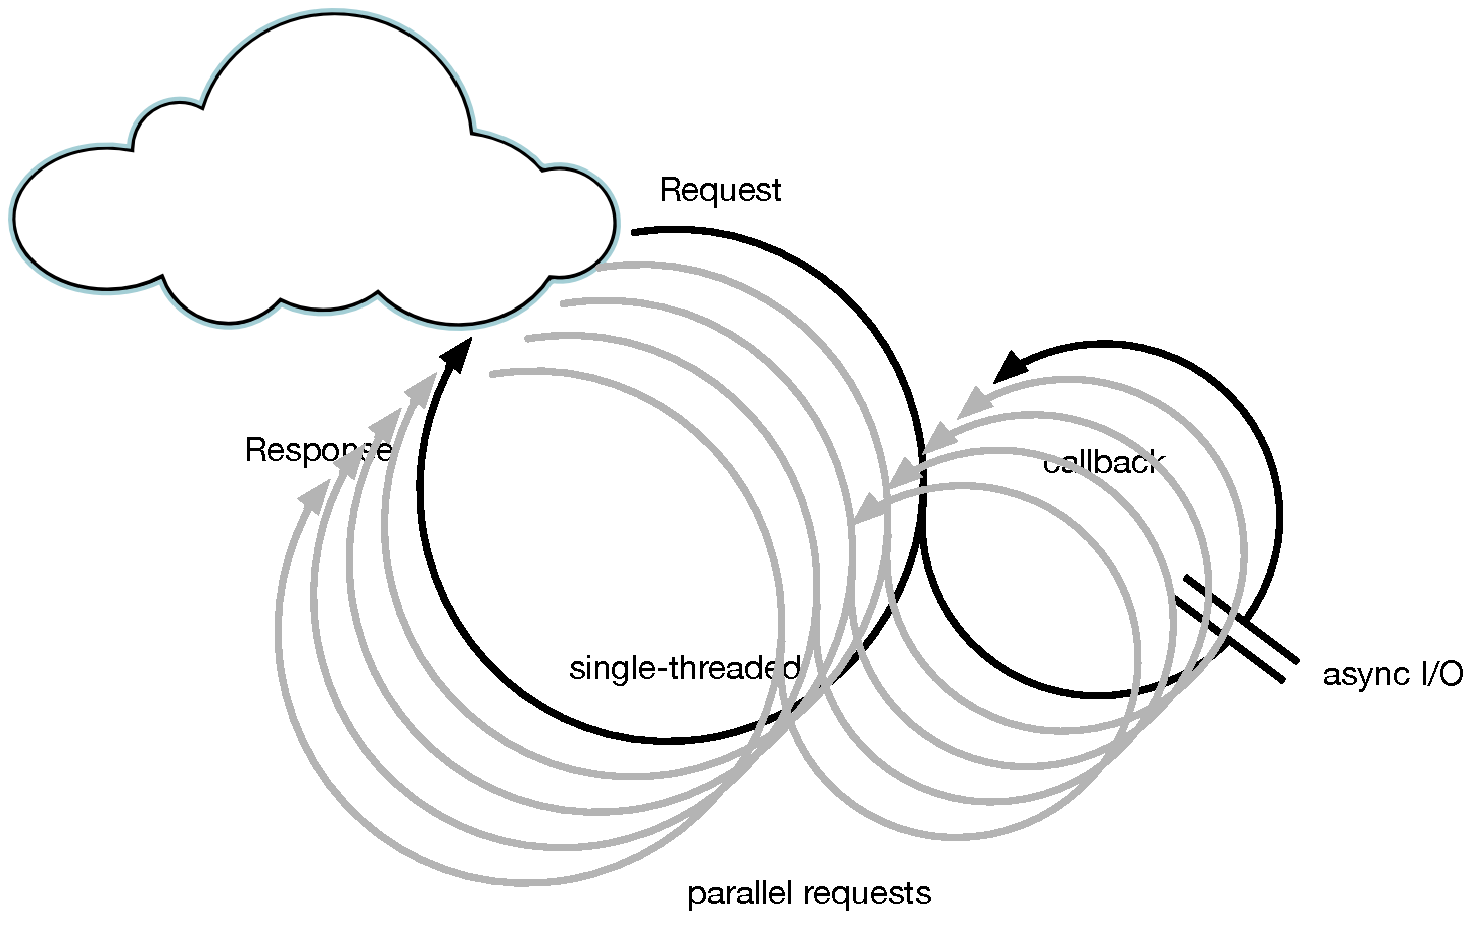
\includegraphics[width=\WIDTH]{../Nodejs4.pdf}
\end{onlyenv}
\end{column}
\hfill 
\begin{column}{.2\textwidth}
\begin{tiny}
\makebox[\textwidth][r]{
\rotatebox{270}{\url{http://blog.mixu.net/2011/02/01/understanding-the-node-js-event-loop/}}
}
\end{tiny}
\end{column}
\end{columns}

\end{frame}

%%%%%%%%%%%%%%%%%%%%%%%%%%%%%%%%%%%%%%%%%%%%%%%%%%
\begin{frame}[fragile]{Mongo DB}

\begin{itemize}
\item No transactions
\item No optimistic locking
\onslide+<2->
\item We implemented optimistic locking ourselves
\end{itemize}

\end{frame}

%%%%%%%%%%%%%%%%%%%%%%%%%%%%%%%%%%%%%%%%%%%%%%%%%%
\begin{frame}[fragile]{Mongo DB}

\begin{center}

\begin{onlyenv}<1>
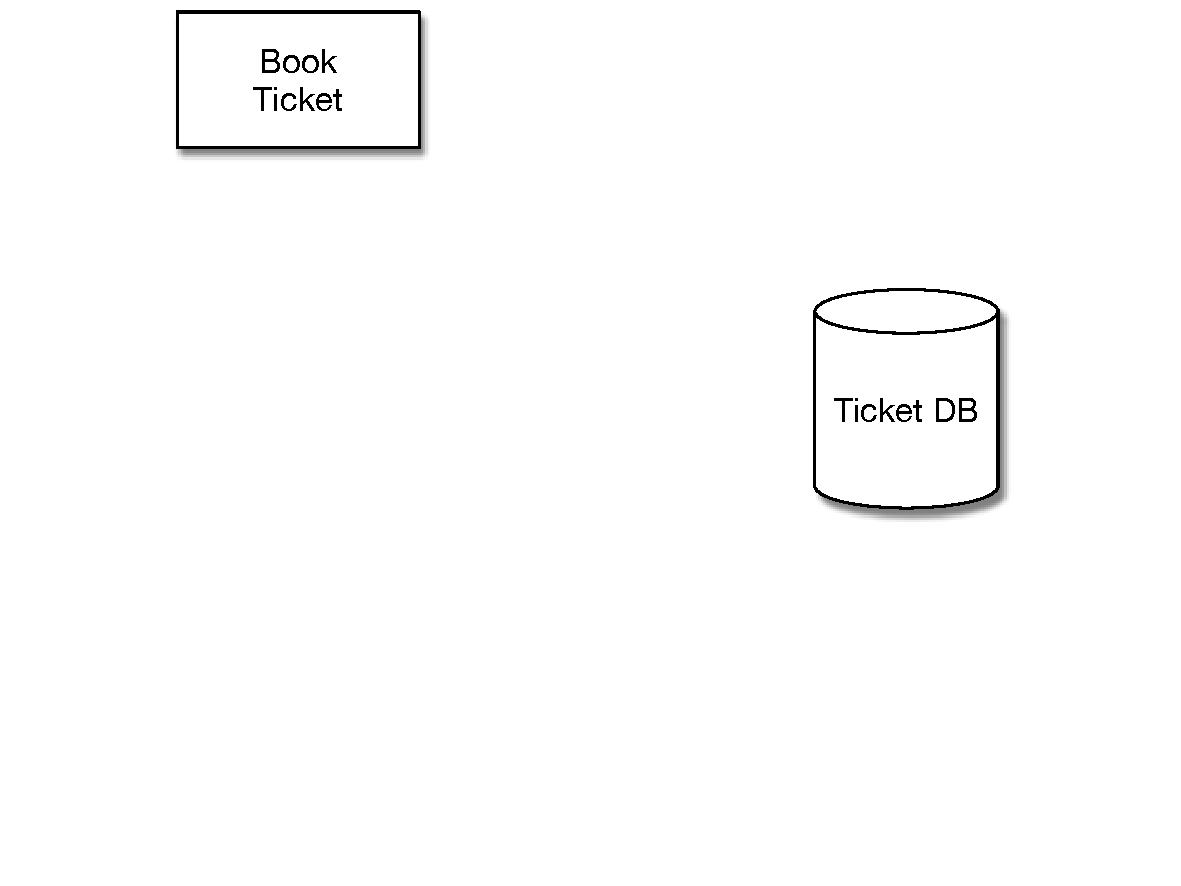
\includegraphics[width=.85\textwidth]{../OptimisticLocking1.pdf}
\end{onlyenv}

\begin{onlyenv}<2>
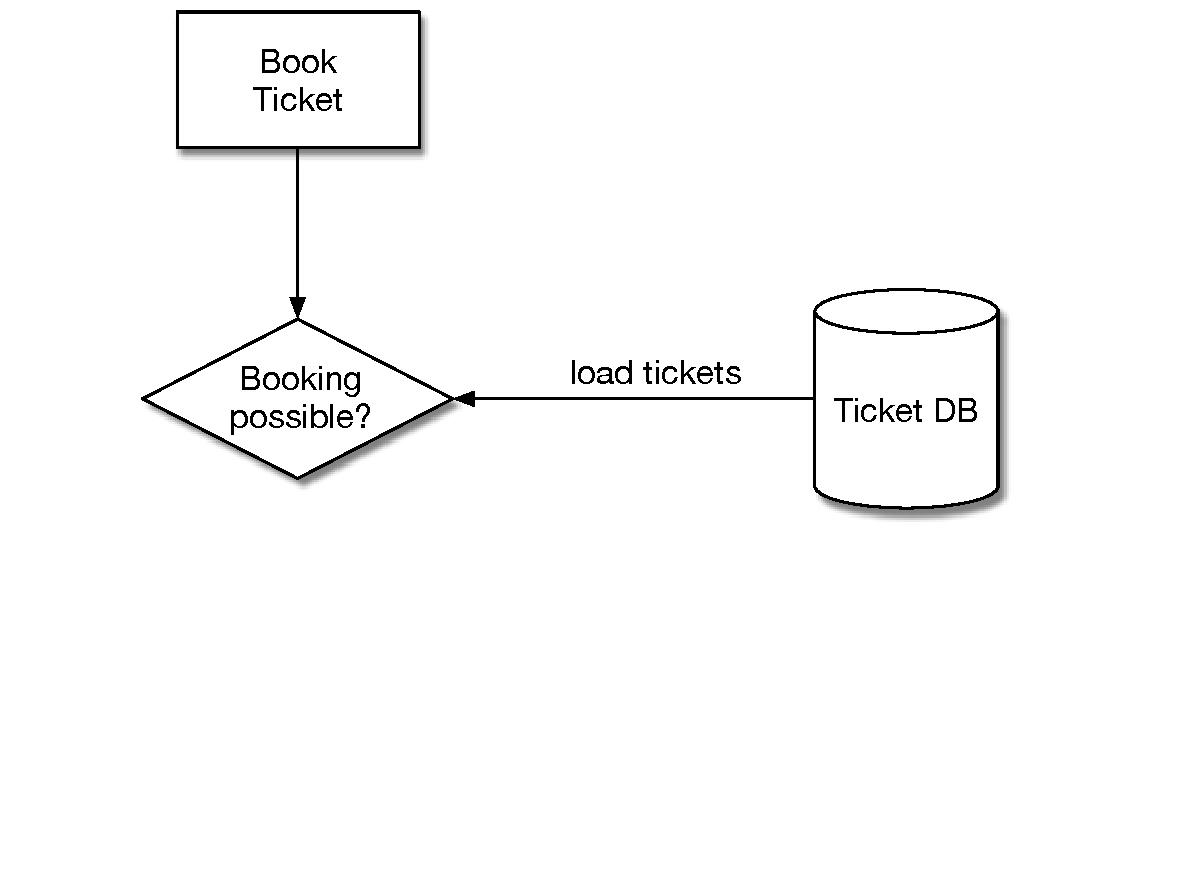
\includegraphics[width=.85\textwidth]{../OptimisticLocking2.pdf}
\end{onlyenv}

\begin{onlyenv}<3>
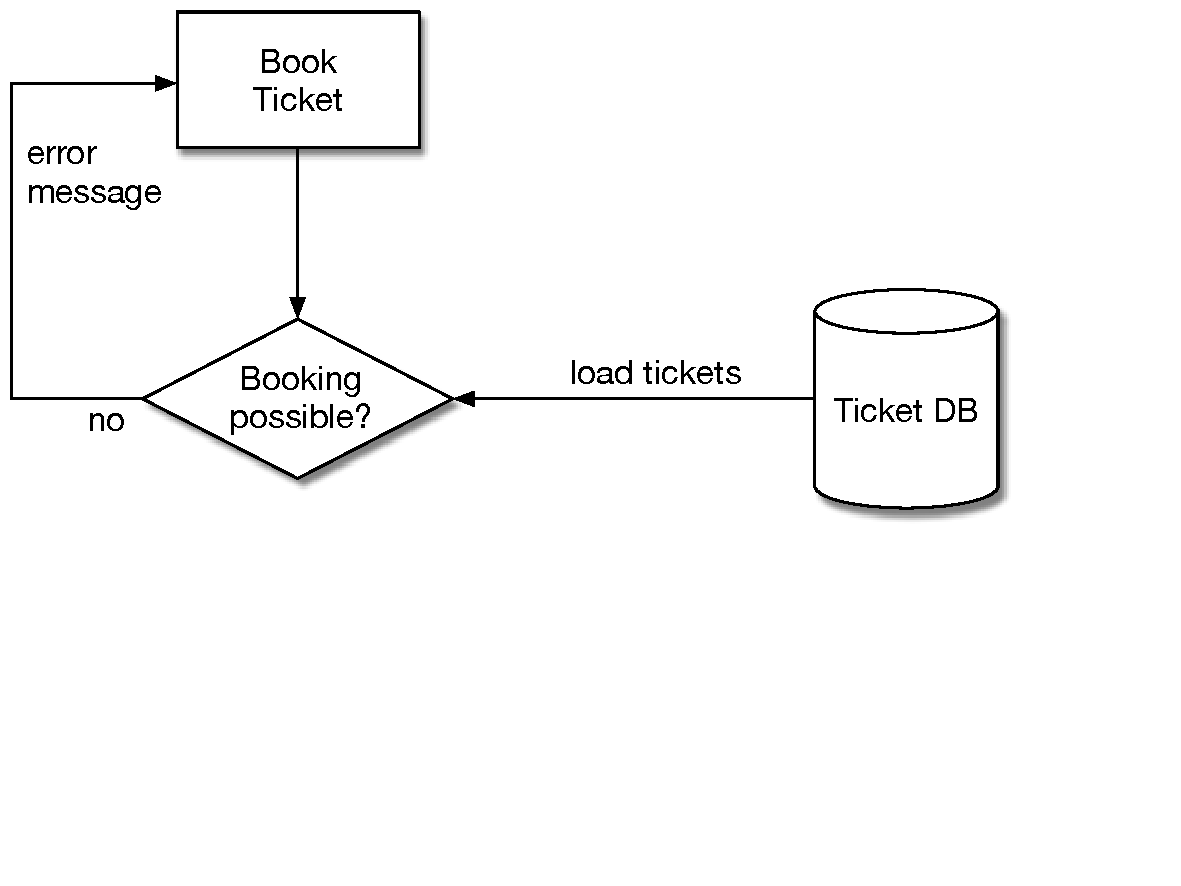
\includegraphics[width=.85\textwidth]{../OptimisticLocking3.pdf}
\end{onlyenv}

\begin{onlyenv}<4>
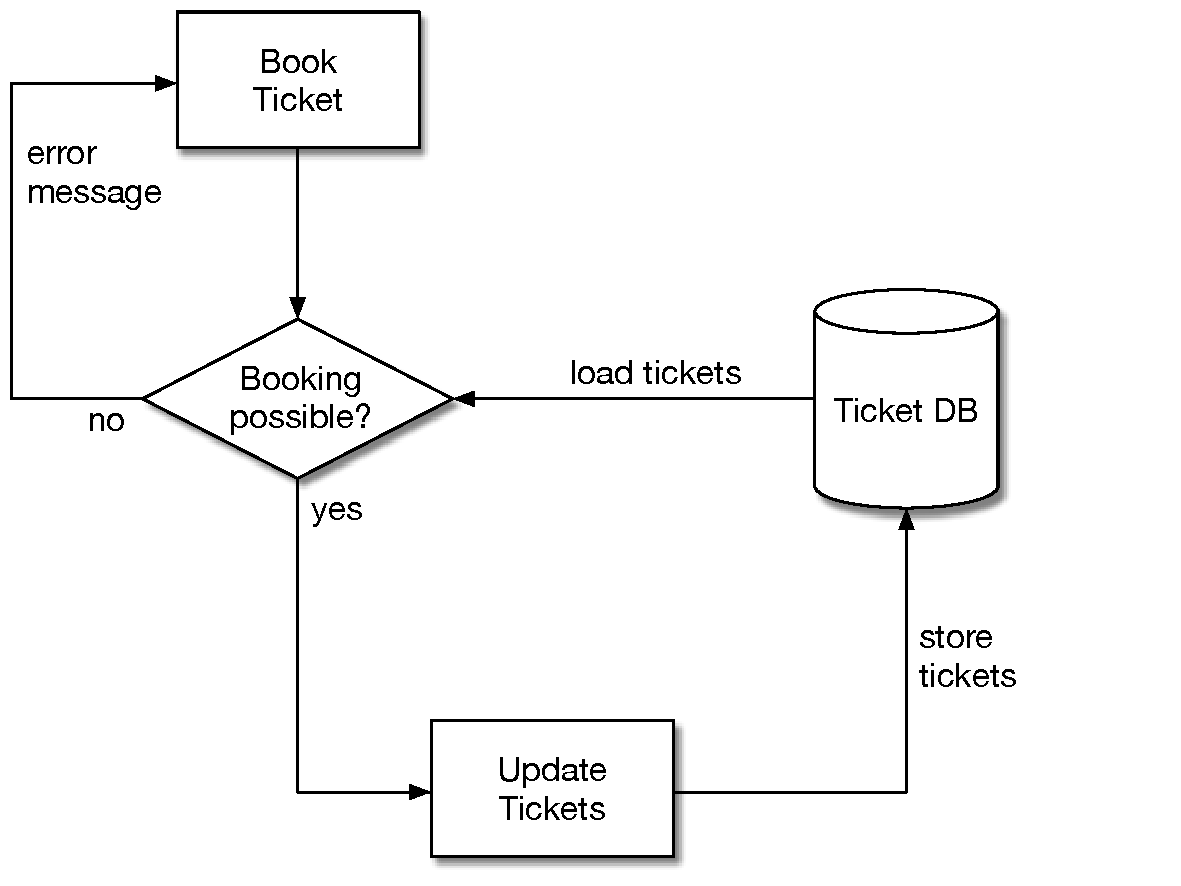
\includegraphics[width=.85\textwidth]{../OptimisticLocking4.pdf}
\end{onlyenv}

\begin{onlyenv}<5>
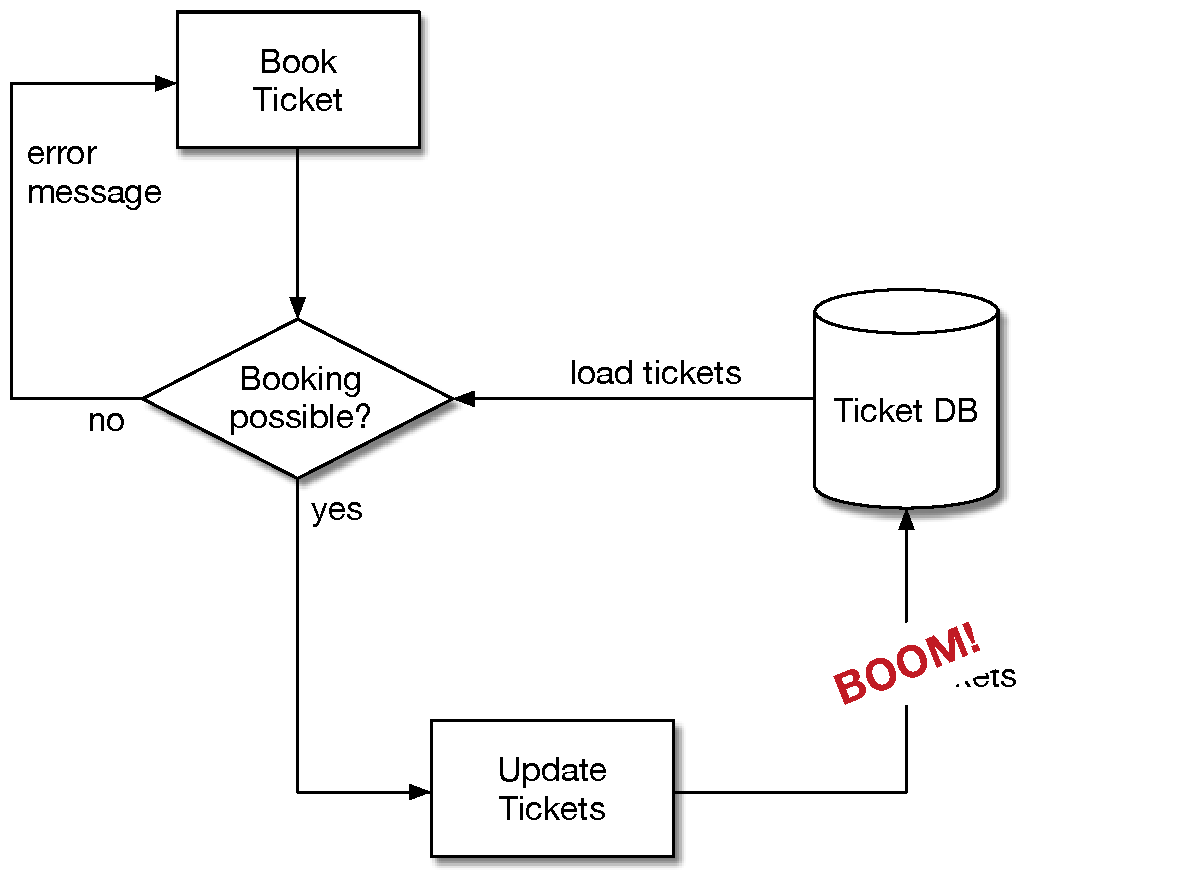
\includegraphics[width=.85\textwidth]{../OptimisticLocking5.pdf}
\end{onlyenv}


\begin{onlyenv}<6>
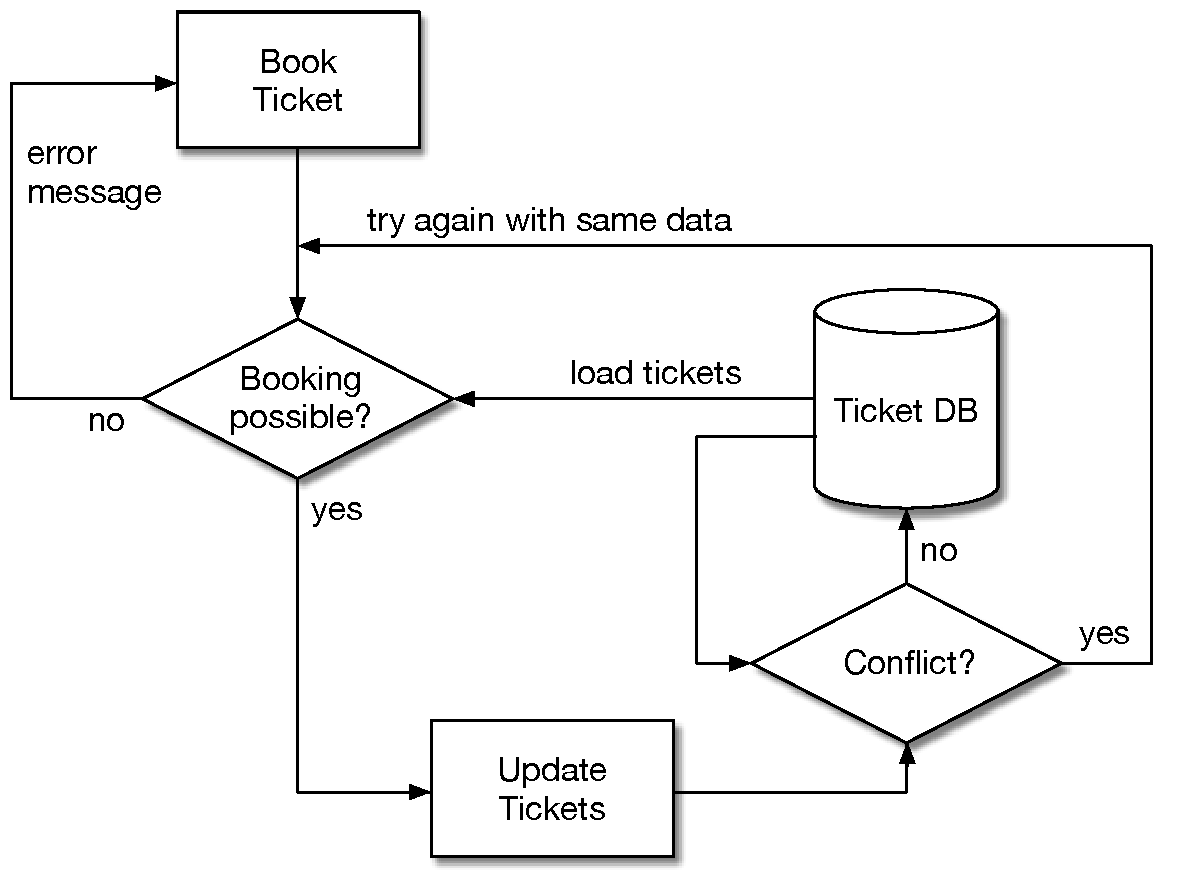
\includegraphics[width=.85\textwidth]{../OptimisticLocking6.pdf}
\end{onlyenv}

\begin{onlyenv}<7>
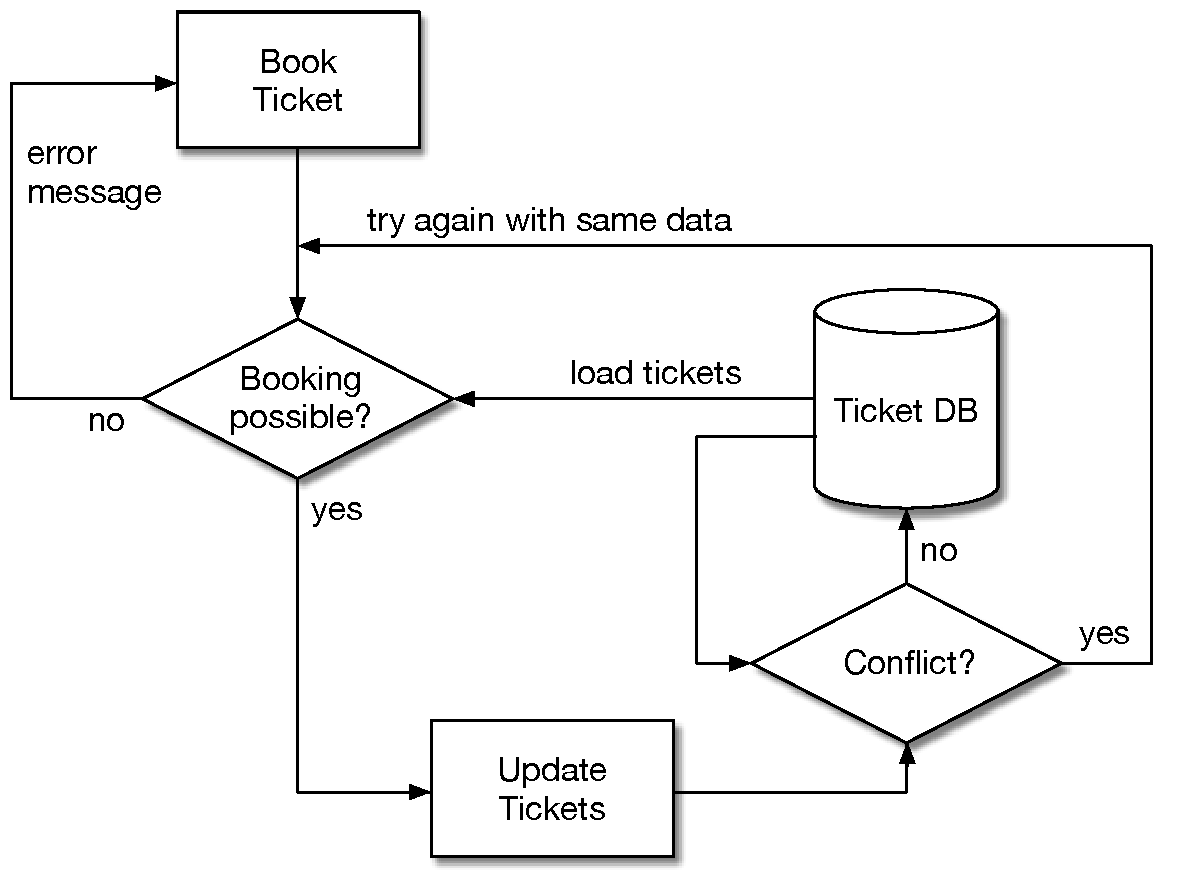
\includegraphics[width=.85\textwidth]{../OptimisticLocking7.pdf}
\end{onlyenv}

\end{center}

\end{frame}

%%%%%%%%%%%%%%%%%%%%%%%%%%%%%%%%%%%%%%%%%%%%%%%%%%
\begin{frame}[fragile]{Our Pre-Event-Sourcing Architecture}

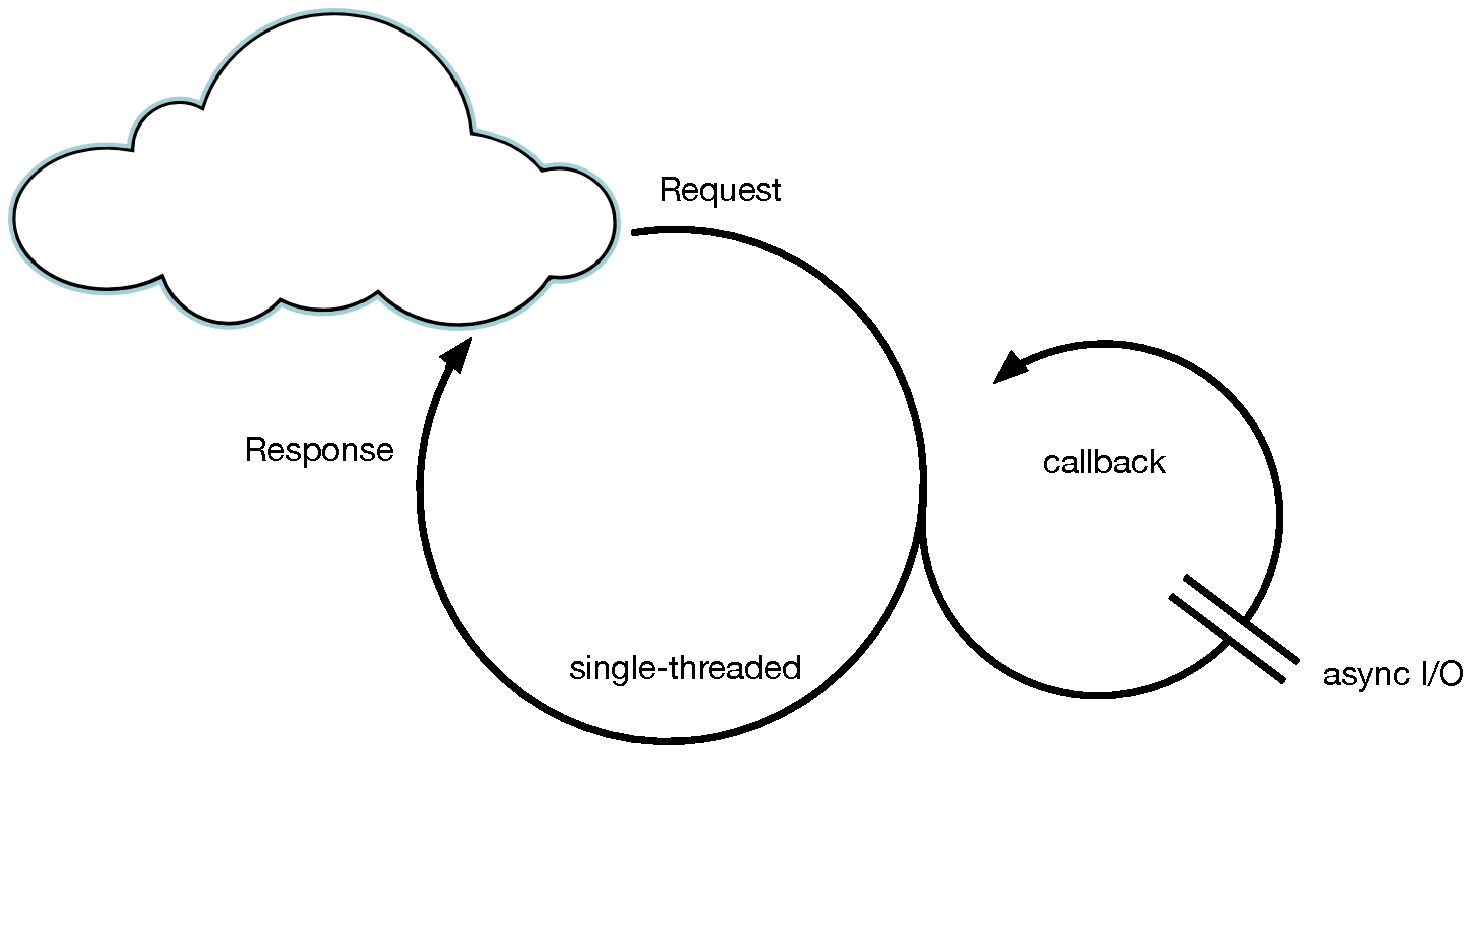
\includegraphics[width=.7\textwidth]{../Nodejs3.pdf}

\begin{itemize}
\item Request comes in, reads \& writes data from/to DB, returns
\item Nothing$^*$ is kept in memory between requests
\end{itemize}

{ \tiny $^*$ Apart from the caching that is done by \texttt{require} }
\end{frame}

%%%%%%%%%%%%%%%%%%%%%%%%%%%%%%%%%%%%%%%%%%%%%%%%%%
\begin{frame}[fragile]{Event Sourcing Without Global State?}

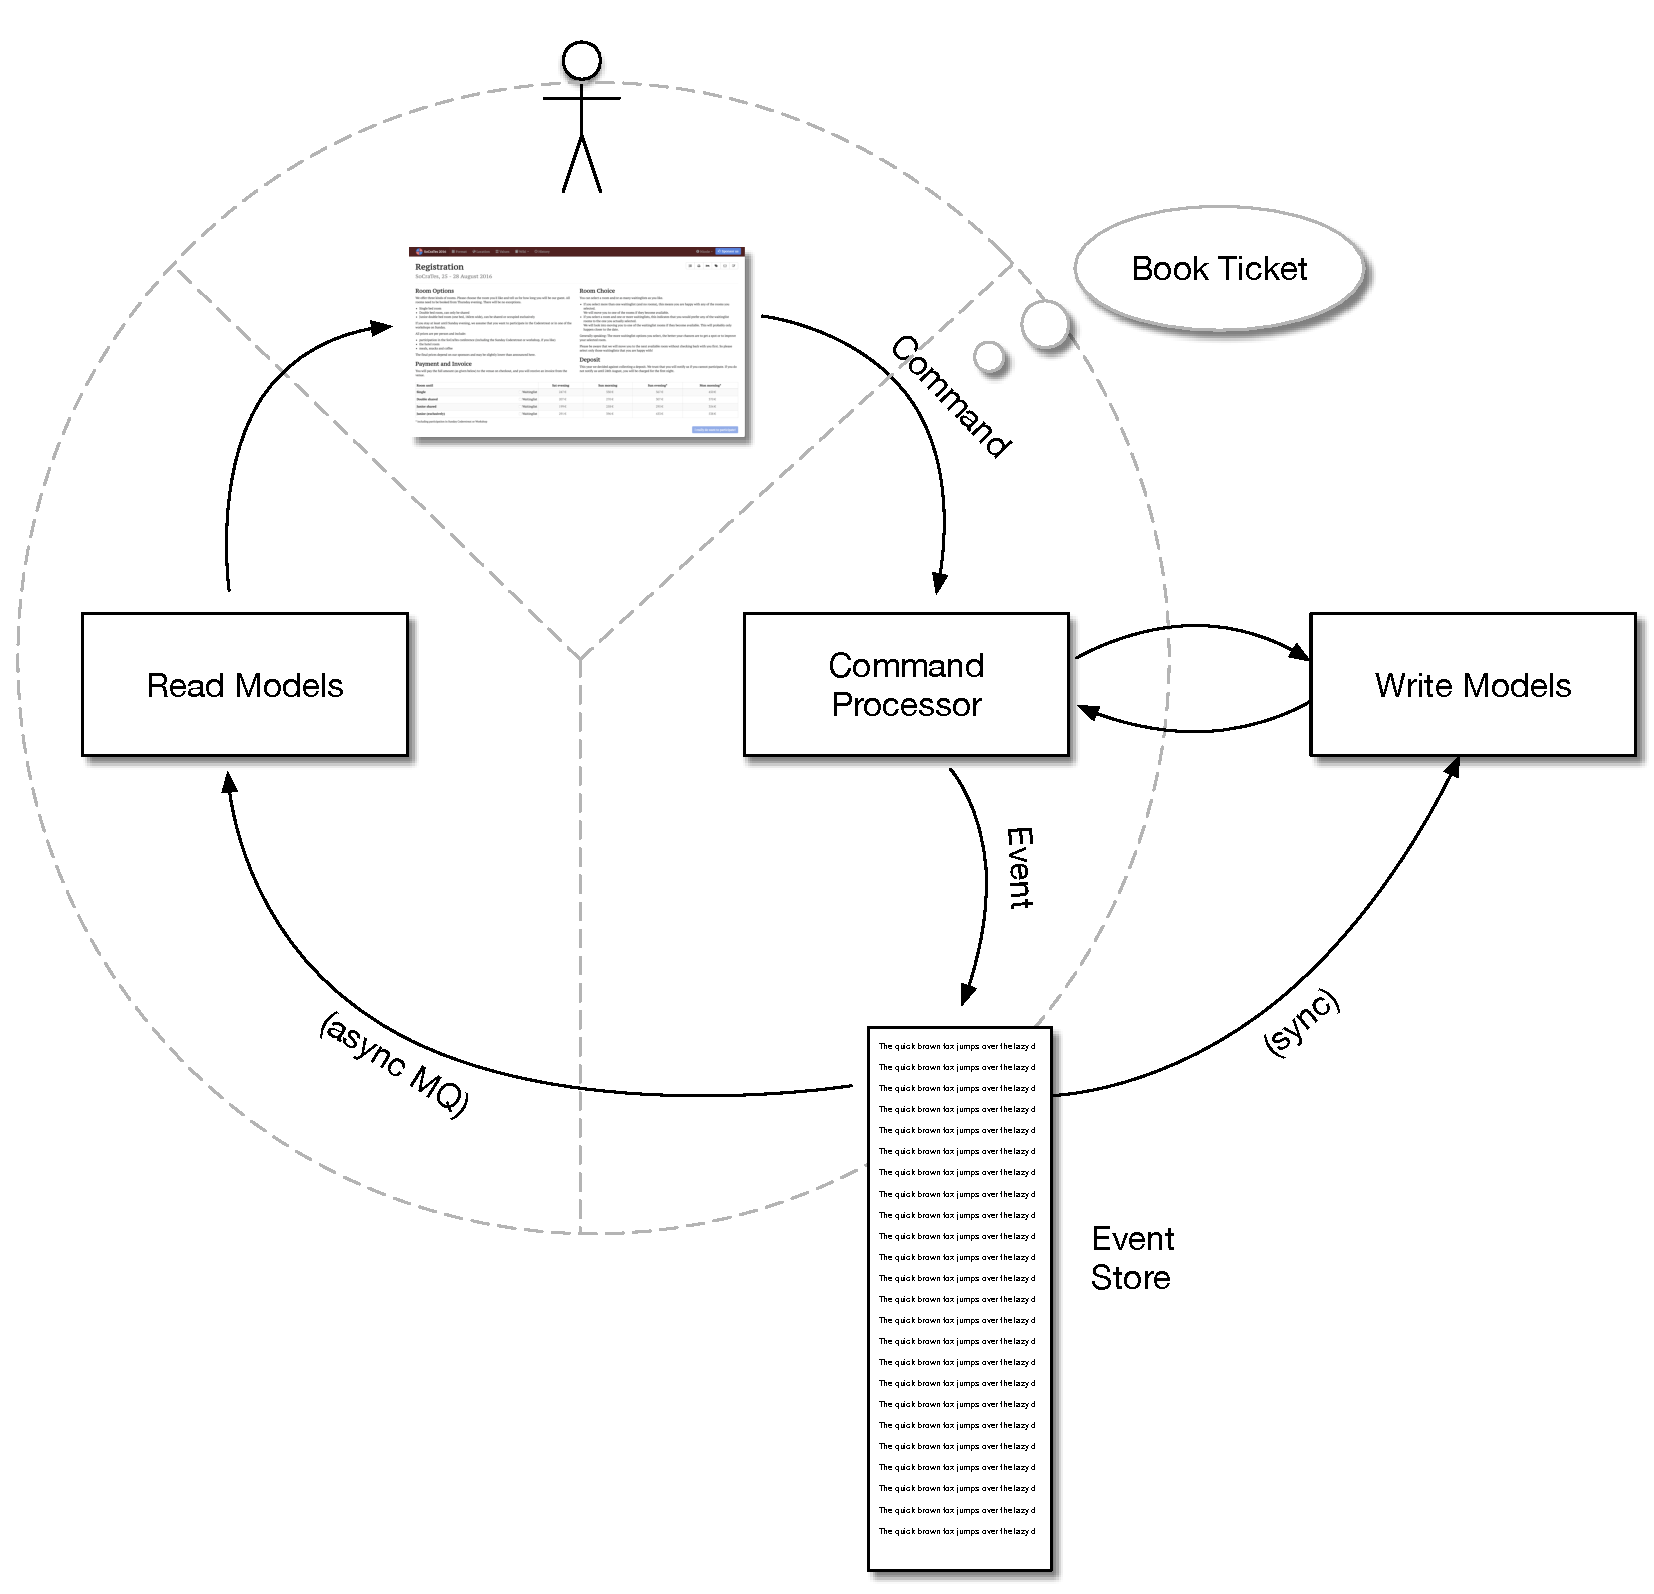
\includegraphics[width=.5\textwidth]{../EventSourcing4.pdf}

\begin{itemize}
\item What about the read and write models?
\end{itemize}

\end{frame}

%%%%%%%%%%%%%%%%%%%%%%%%%%%%%%%%%%%%%%%%%%%%%%%%%%
\begin{frame}[fragile]{Working Hypothesis}

\textbf{Rough Estimations:} \\[.7em]
We expected a couple hundred events altogether

\onslide+<2->
\vspace{5em}

\textbf{Working Hypothesis:} \\[.7em]
We can hydrate the models from the eventstore on each request

\end{frame}


%%%%%%%%%%%%%%%%%%%%%%%%%%%%%%%%%%%%%%%%%%%%%%%%%%
\begin{frame}[fragile]{What was going on?}

\renewcommand{\SPACE}{.6em}

Remember: 2-phase registration (reservation $\rightarrow$ registration)
\vspace{\SPACE}

\onslide+<2->
First user came in:
\vspace{\SPACE}

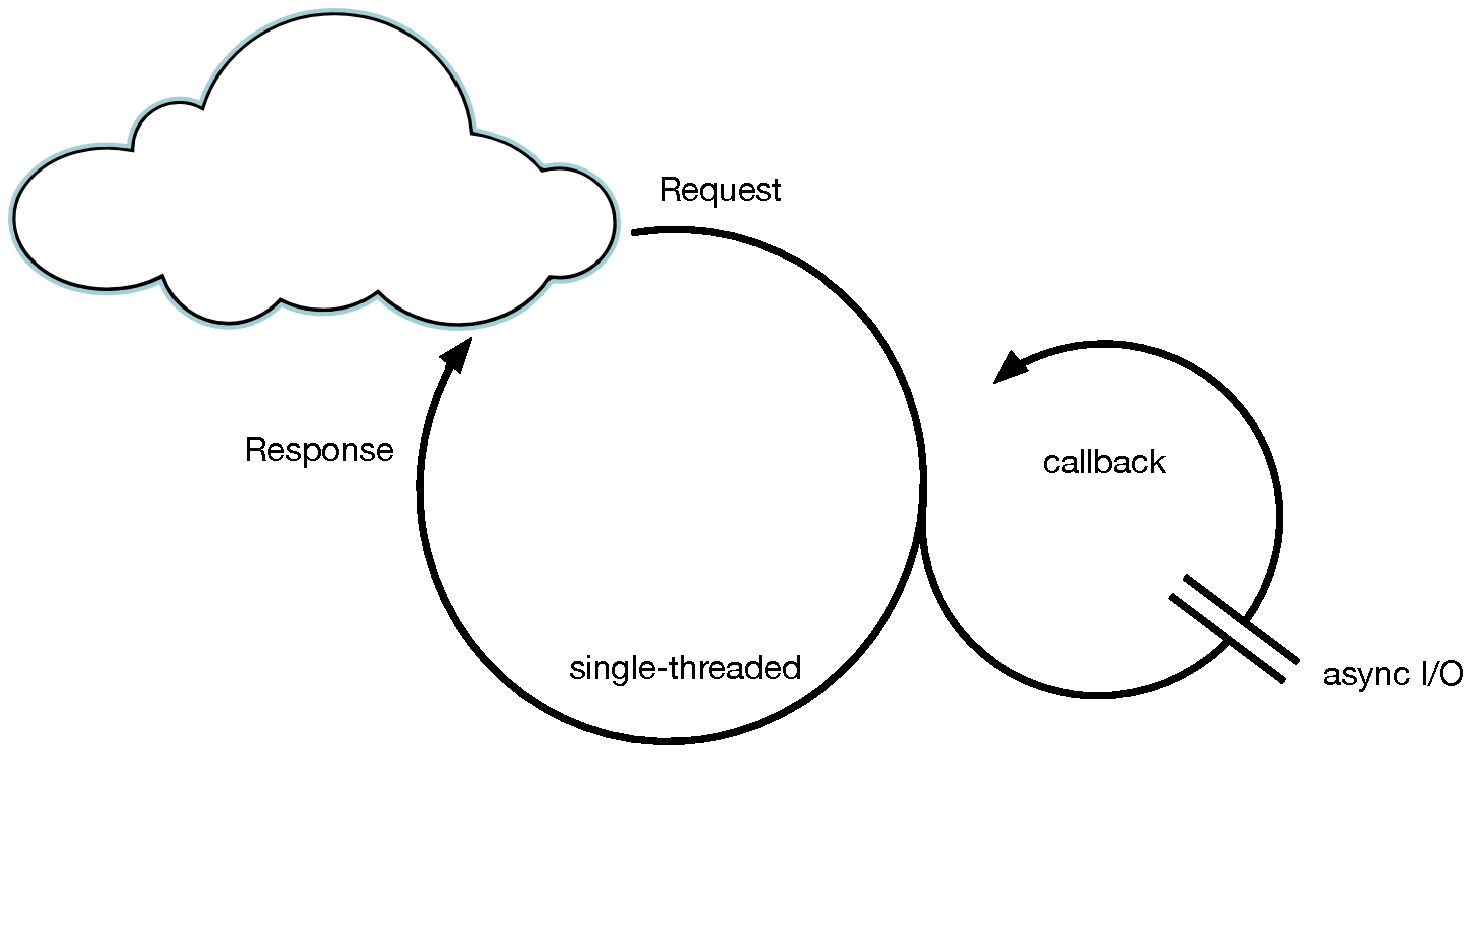
\includegraphics[width=.5\textwidth]{../Nodejs3.pdf}

\onslide+<3->
Reading from DB parallelized it, so more users came in and read from DB

\end{frame}

%%%%%%%%%%%%%%%%%%%%%%%%%%%%%%%%%%%%%%%%%%%%%%%%%%
\begin{frame}[fragile]{What was going on?}

\renewcommand{\SPACE}{1em}

\begin{center}

\begin{onlyenv}<1>
First user was able to persist her reservation:
\vspace{\SPACE}

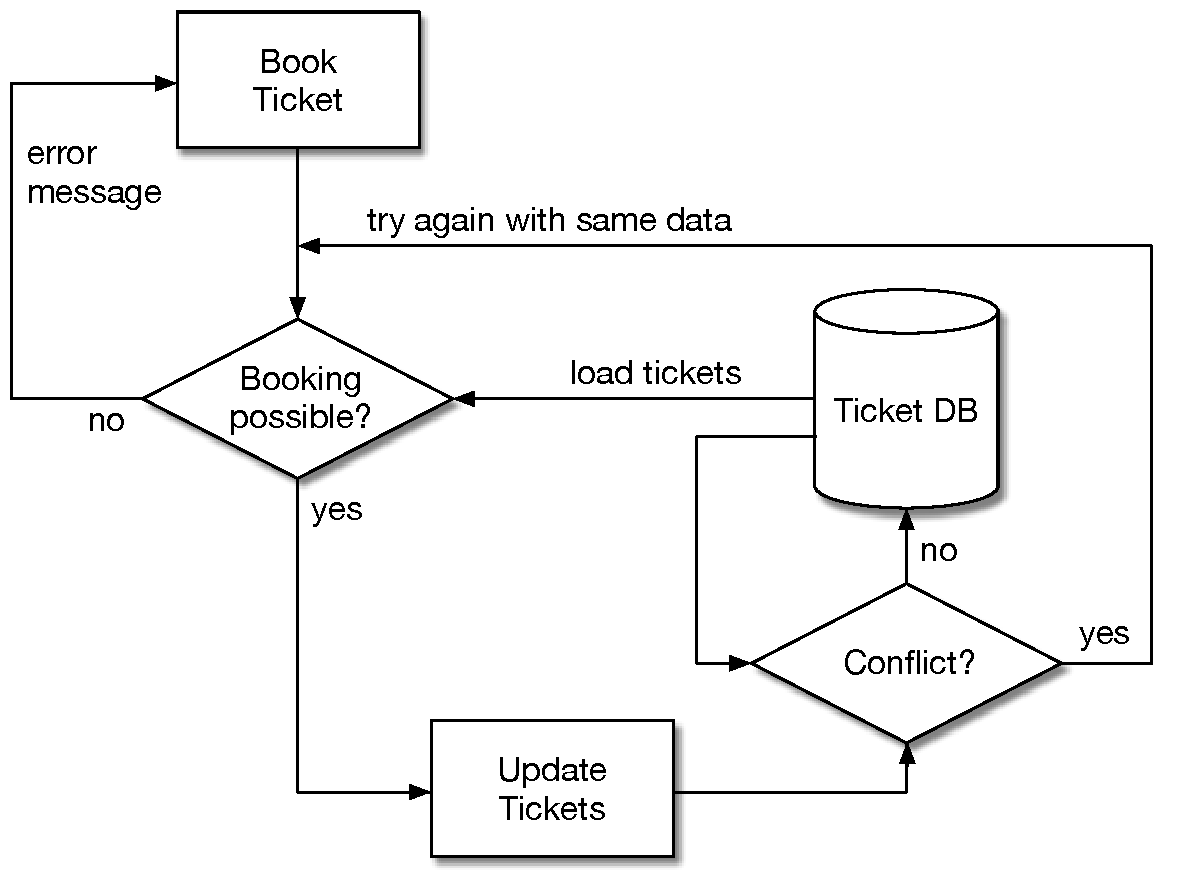
\includegraphics[width=.6\textwidth]{../OptimisticLocking6.pdf}
\end{onlyenv}

\begin{onlyenv}<2>
All subsequent users produced conflicts: 
\vspace{\SPACE}

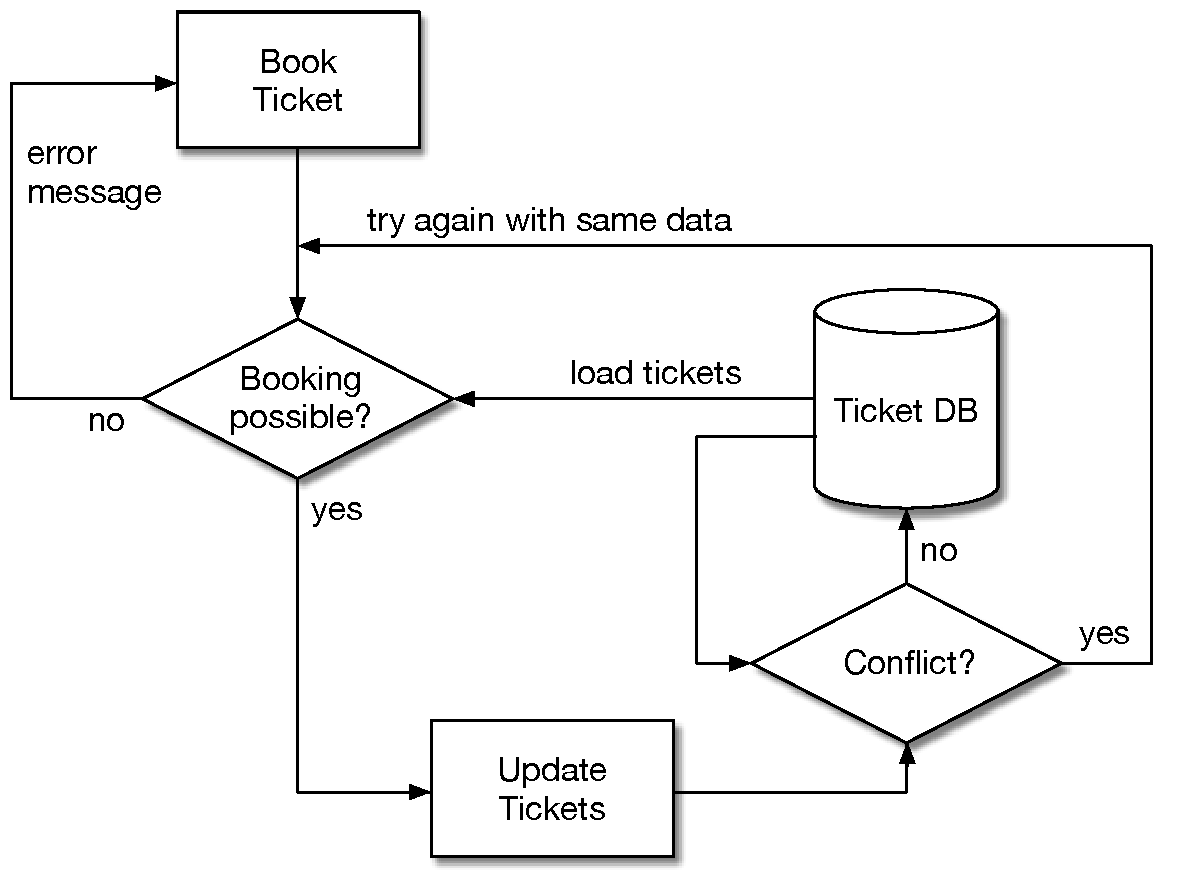
\includegraphics[width=.6\textwidth]{../OptimisticLocking7.pdf}
\end{onlyenv}

\begin{onlyenv}<3>
And retried...
\vspace{\SPACE}

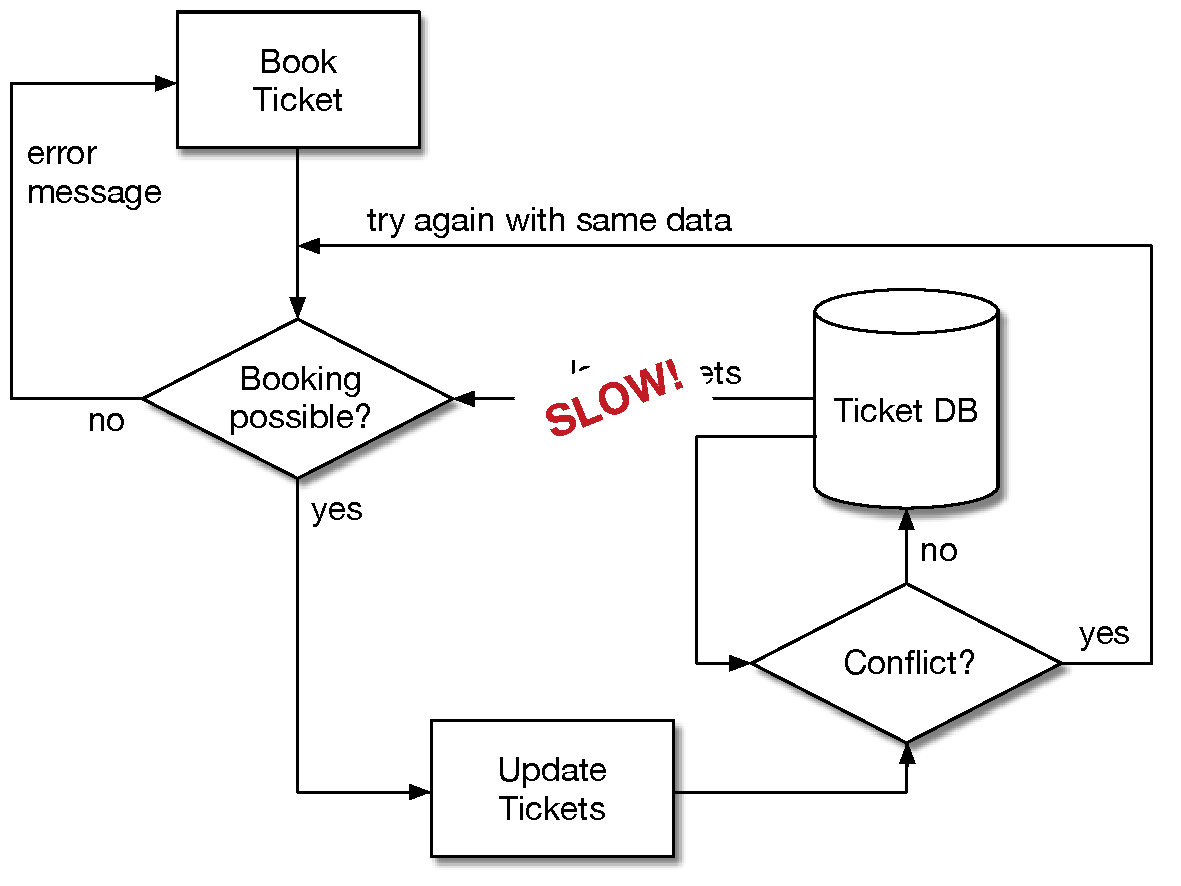
\includegraphics[width=.6\textwidth]{../OptimisticLocking8.pdf}
\end{onlyenv}

\begin{onlyenv}<4>
And got conflicts again...
\vspace{\SPACE}

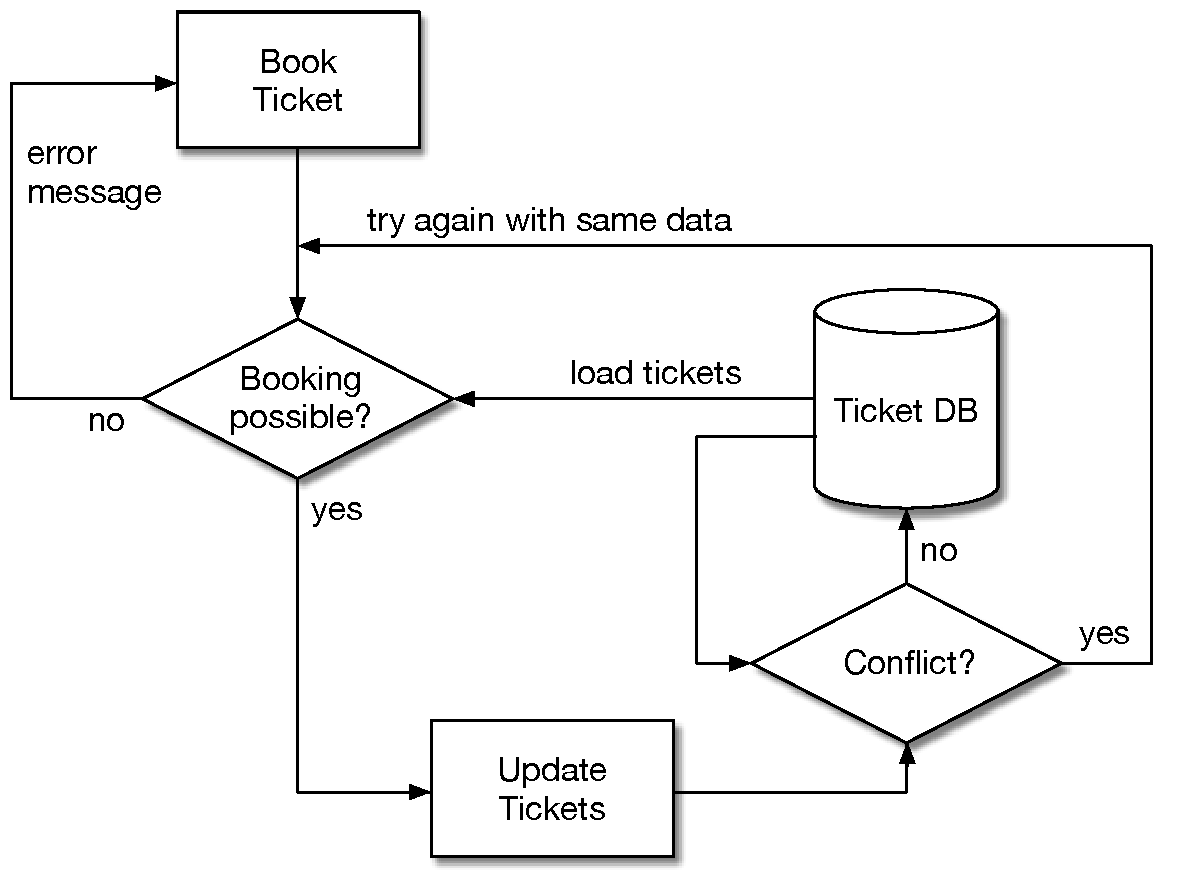
\includegraphics[width=.6\textwidth]{../OptimisticLocking7.pdf}
\end{onlyenv}

\begin{onlyenv}<5>
And retried again...
\vspace{\SPACE}

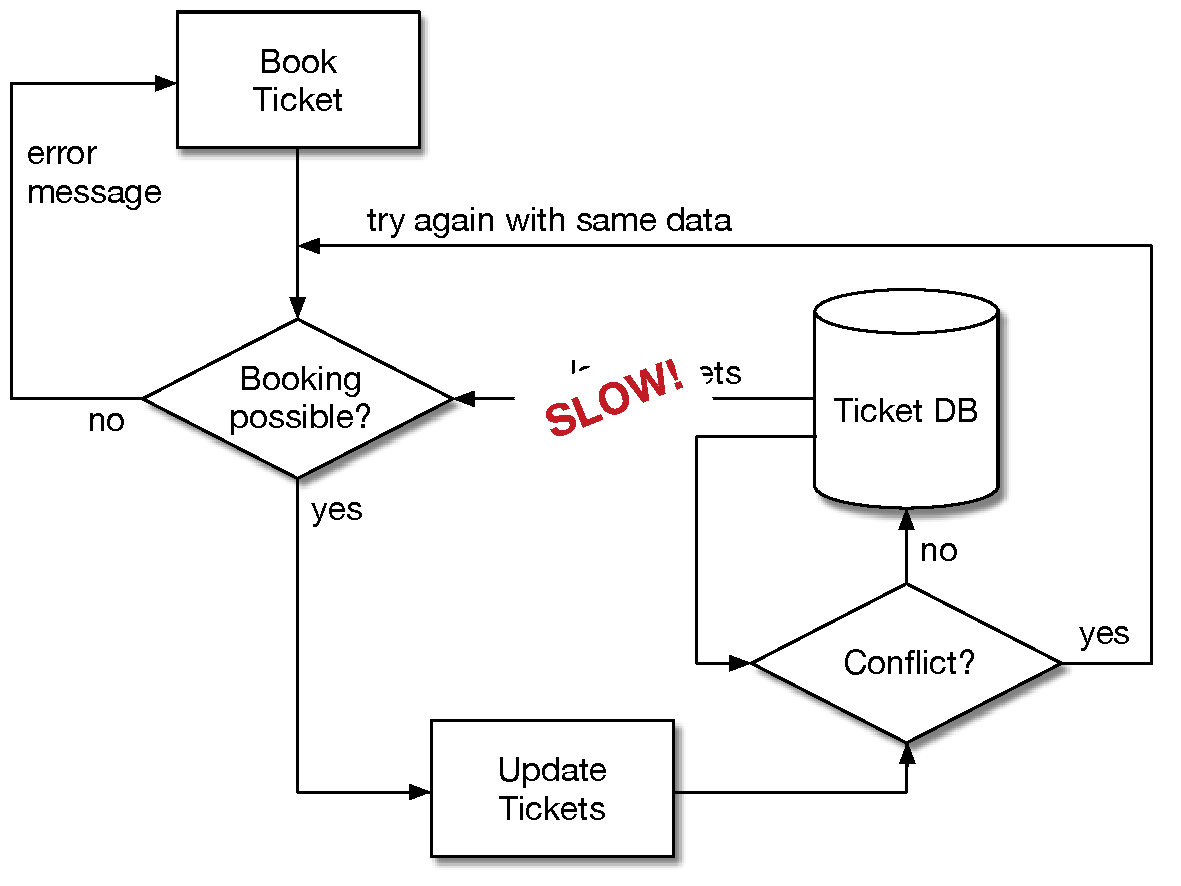
\includegraphics[width=.6\textwidth]{../OptimisticLocking8.pdf}
\end{onlyenv}

\begin{onlyenv}<6>
\renewcommand{\SPACE}{3em}

Slow hydrating on read
\vspace{\SPACE}

$\Longrightarrow$ Huge number of parallel requests
\vspace{\SPACE}

$\Longrightarrow$ Self-propelling disaster.
\end{onlyenv}

\end{center}

\end{frame}

%%%%%%%%%%%%%%%%%%%%%%%%%%%%%%%%%%%%%%%%%%%%%%%%%%
\begin{frame}[fragile]{The End}

After 25 minutes, I shut down the server.
                  
\onslide+<2->
                  
\vspace{3em}

~ \hspace{10em} Nobody had been able to register.
                  
\end{frame}

%%%%%%%%%%%%%%%%%%%%%%%%%%%%%%%%%%%%%%%%%%%%%%%%%%
\begin{frame}[fragile]{Problem I}

Hydrating the read and write models takes longer than we had expected.
                  
\onslide+<2->
                  
\vspace{3em}

$\Longrightarrow$ We must cache the read and write models.
                  
\end{frame}

%%%%%%%%%%%%%%%%%%%%%%%%%%%%%%%%%%%%%%%%%%%%%%%%%%
\begin{frame}[fragile]{Caching the Global EventStore}

\renewcommand{\SPACE}{-0.9em}

\onslide+<1->
\begin{highlight}{1}
function getGlobalEventStoreForWriting(url, callback) {
\end{highlight}
%%
\onslide+<2->
\vspace{\SPACE}
\begin{highlight}{2}
  const cacheKey = keyFor(url, GLOBAL_EVENT_STORE_FOR_WRITING);
  const cachedStore = cache.get(cacheKey);
  if (cachedStore) {
    return callback(null, cachedStore);
  }
\end{highlight}
%%
\onslide+<3->
\vspace{\SPACE}
\begin{highlight}{3}
  mongo_async.getEventStore(url, function (err, eventStore) {
    if (err || !eventStore) { return callback(err); }
\end{highlight}
%%
\onslide+<4->
\vspace{\SPACE}
\begin{highlight}{4}
    const cachedWhileFetching = cache.get(cacheKey);
    if (cachedWhileFetching) {
      return callback(null, cachedWhileFetching);
    }
\end{highlight}
%%
\onslide+<5->
\vspace{\SPACE}
\begin{highlight}{5}
    cache.set(cacheKey, eventStore);
    callback(null, eventStore);
\end{highlight}
%%
\onslide+<3->
\vspace{\SPACE}
\begin{highlight}{3}
  });
\end{highlight}
%%
\onslide+<1->
\vspace{\SPACE}
\begin{highlight}{1}
}
\end{highlight}


\end{frame}



%%%%%%%%%%%%%%%%%%%%%%%%%%%%%%%%%%%%%%%%%%%%%%%%%%
\begin{frame}[fragile]{``True'' Event Sourcing and Our Adaptation}

\begin{center}

\begin{onlyenv}<1>
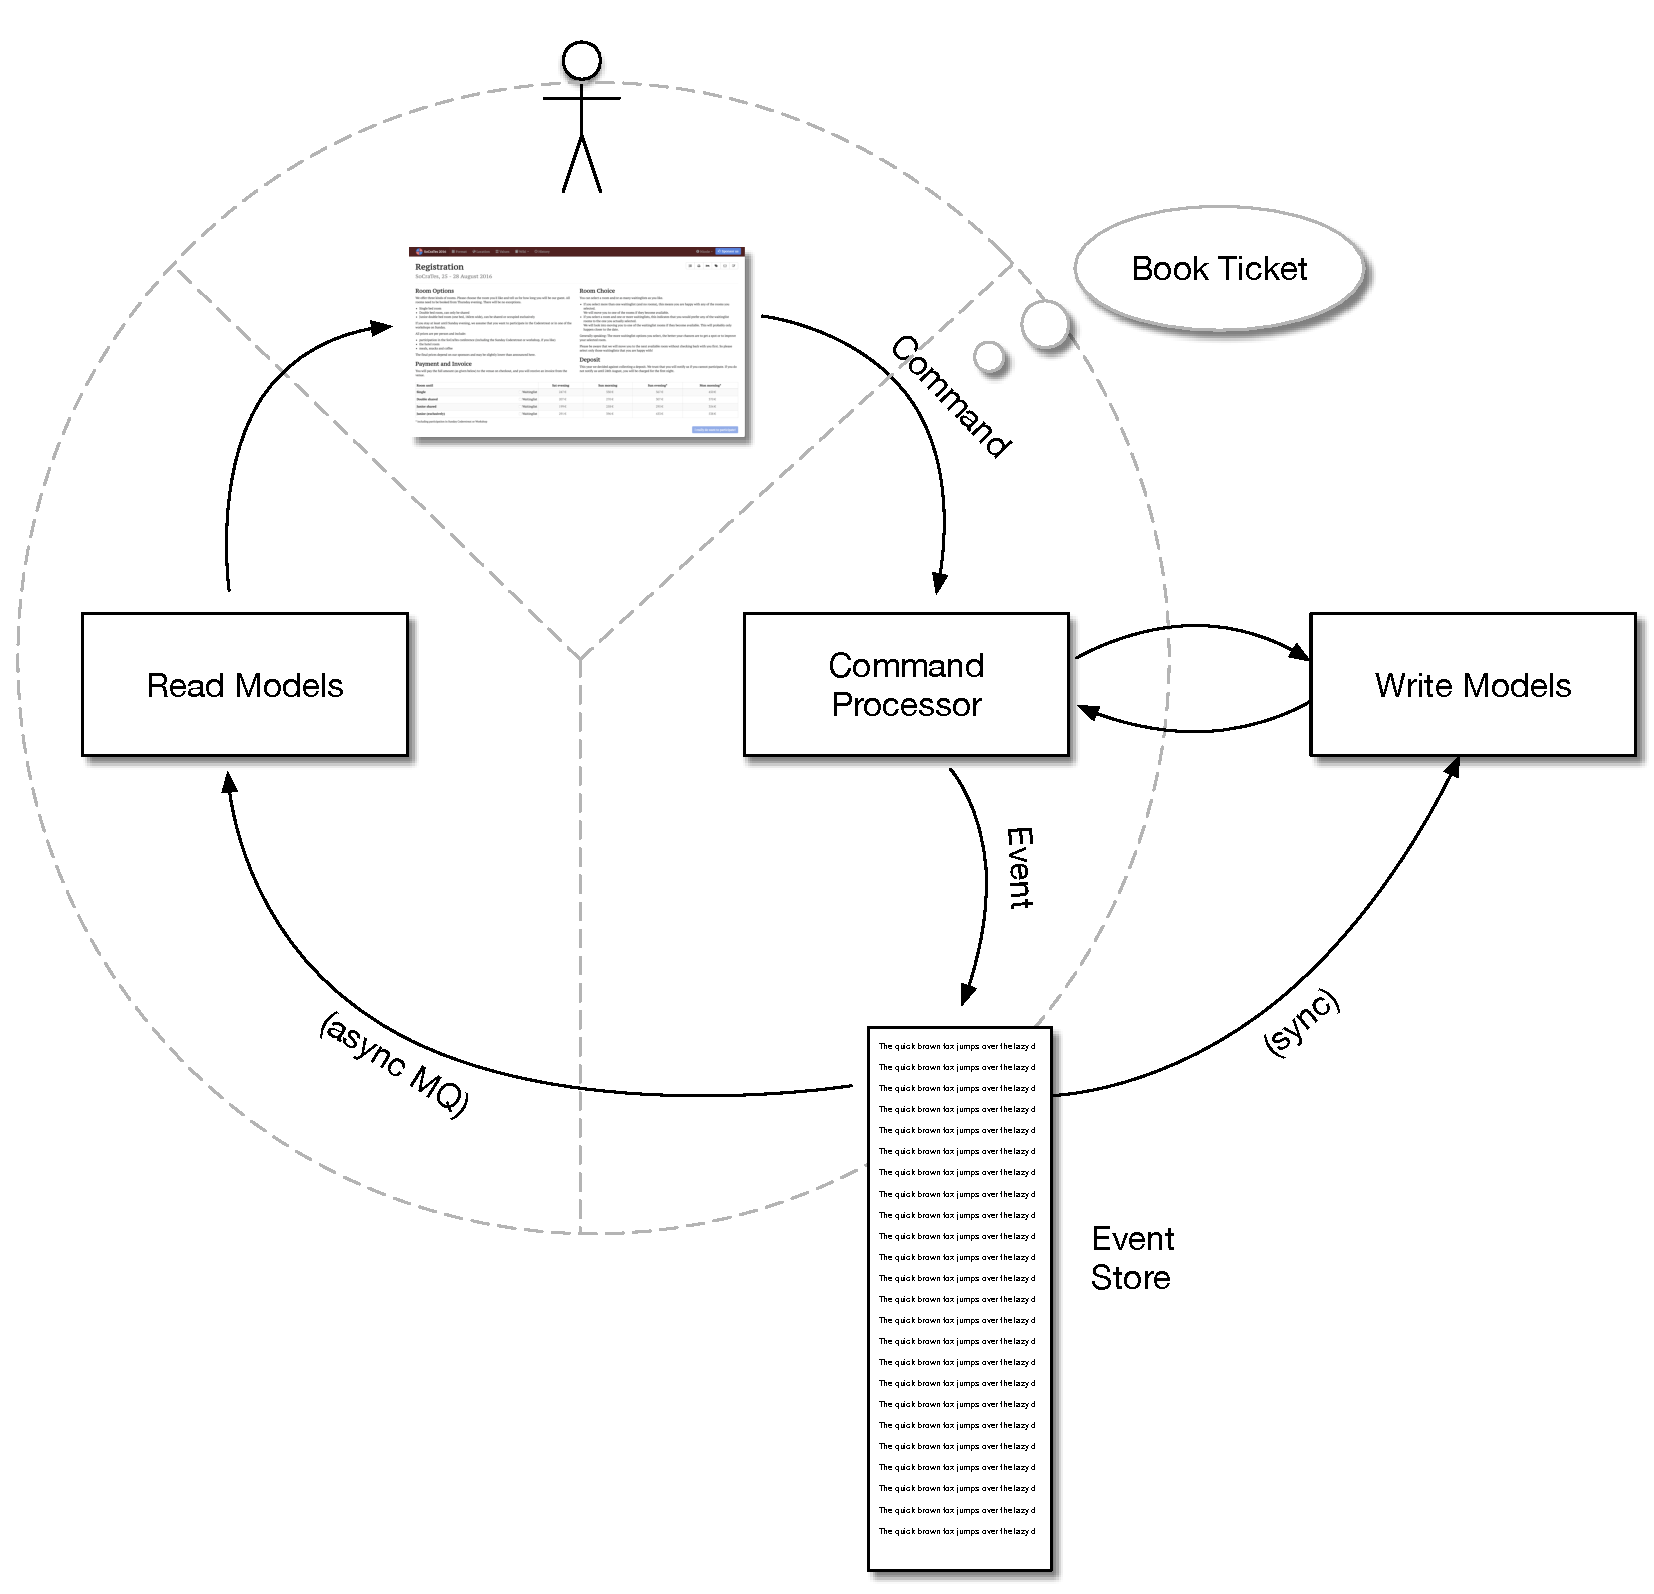
\includegraphics[width=.7\textwidth]{../EventSourcing4.pdf}
\end{onlyenv}

\begin{onlyenv}<2>
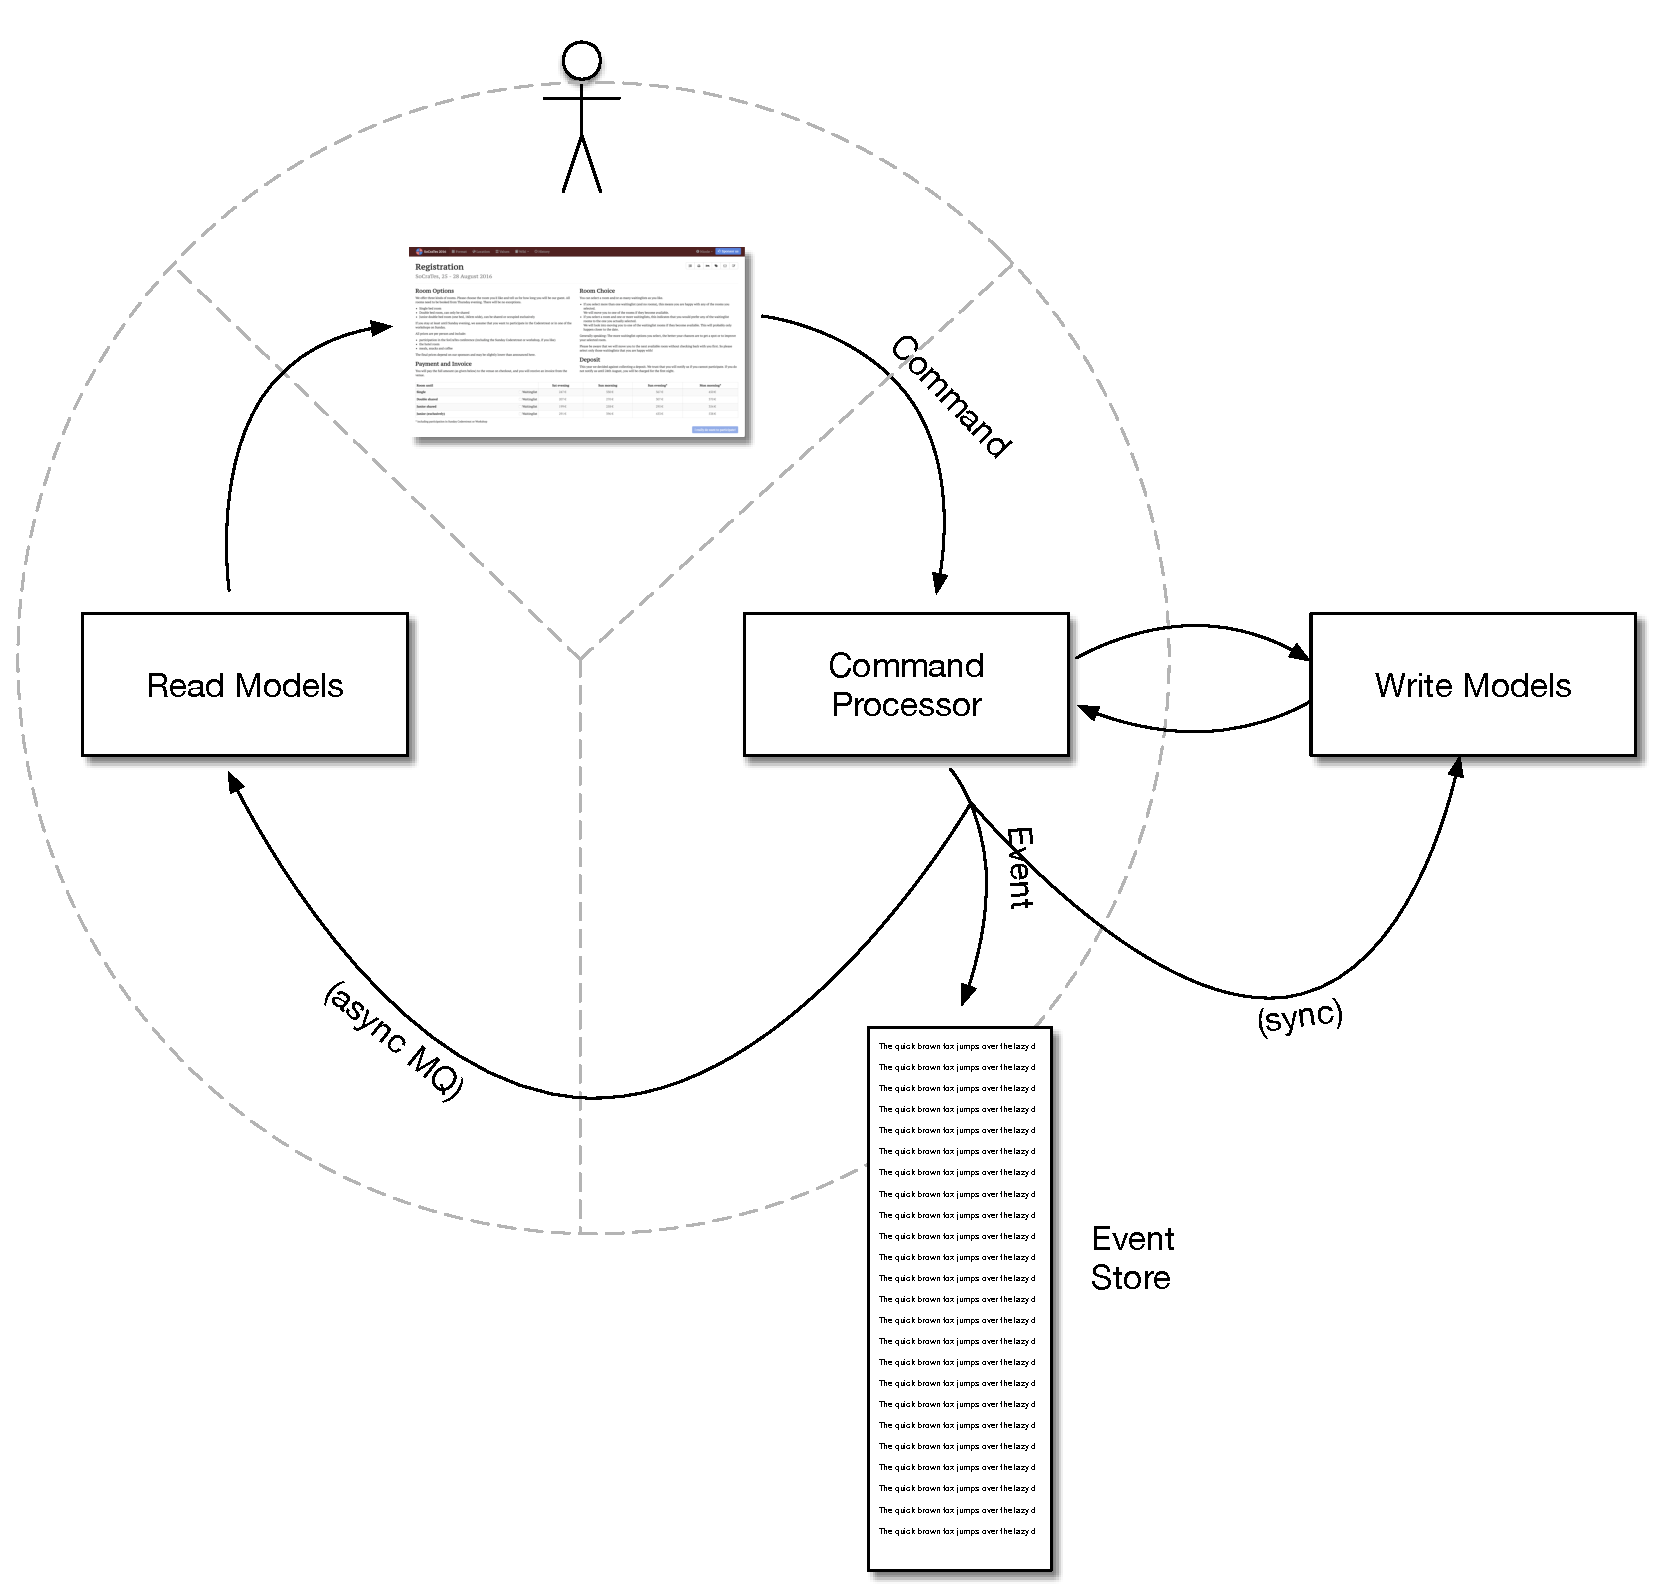
\includegraphics[width=.7\textwidth]{../EventSourcingOurStyle.pdf}
\end{onlyenv}


\begin{onlyenv}<3>

\textbf{Important:}

\vspace{4em}
Persisting the event store must be the \textbf{last} action to avoid parallelization!
\end{onlyenv}

\end{center}

\end{frame}

%%%%%%%%%%%%%%%%%%%%%%%%%%%%%%%%%%%%%%%%%%%%%%%%%%
\begin{frame}[fragile]{Caching the Read Models}

\renewcommand{\SPACE}{-0.9em}

\onslide+<1->
\begin{highlight}{1}
function getReadModel(url, key, ReadModel, callback) {
\end{highlight}
%%
\onslide+<2->
\vspace{\SPACE}
\begin{highlight}{2}
  const cacheKey = keyFor(url, key);
  var cachedModel = cache.get(cacheKey);
  if (cachedModel) {
    return callback(null, cachedModel);
  }
\end{highlight}
%%
\onslide+<3->
\vspace{\SPACE}
\begin{highlight}{3}
  mongo_async.getEventStore(url, function (err, eventStore) {
    if (err || !eventStore) { return callback(err); }
\end{highlight}
%%
\onslide+<4->
\vspace{\SPACE}
\begin{highlight}{4}
    var cachedWhileFetching = cache.get(cacheKey);
    if (cachedWhileFetching) {
      return callback(null, cachedWhileFetching);
    }
\end{highlight}
%%
\onslide+<5->
\vspace{\SPACE}
\begin{highlight}{5}
    const newModel = new ReadModel(eventStore);
    cache.set(cacheKey, newModel);
    callback(null, newModel);
\end{highlight}
%%
\onslide+<3->
\vspace{\SPACE}
\begin{highlight}{3}
  });
\end{highlight}
%%
\onslide+<1->
\vspace{\SPACE}
\begin{highlight}{1}
}
\end{highlight}

\end{frame}


%%%%%%%%%%%%%%%%%%%%%%%%%%%%%%%%%%%%%%%%%%%%%%%%%%
\begin{frame}[fragile]{Problem II}

Parallelization leads to write conflicts

\onslide+<2->
                  
\vspace{3em}

$\Longrightarrow$ We must eliminate parallelization.

\end{frame}

%%%%%%%%%%%%%%%%%%%%%%%%%%%%%%%%%%%%%%%%%%%%%%%%%%
\begin{frame}[fragile]{Eliminating Parallelization}

\begin{center}

\begin{onlyenv}<1>
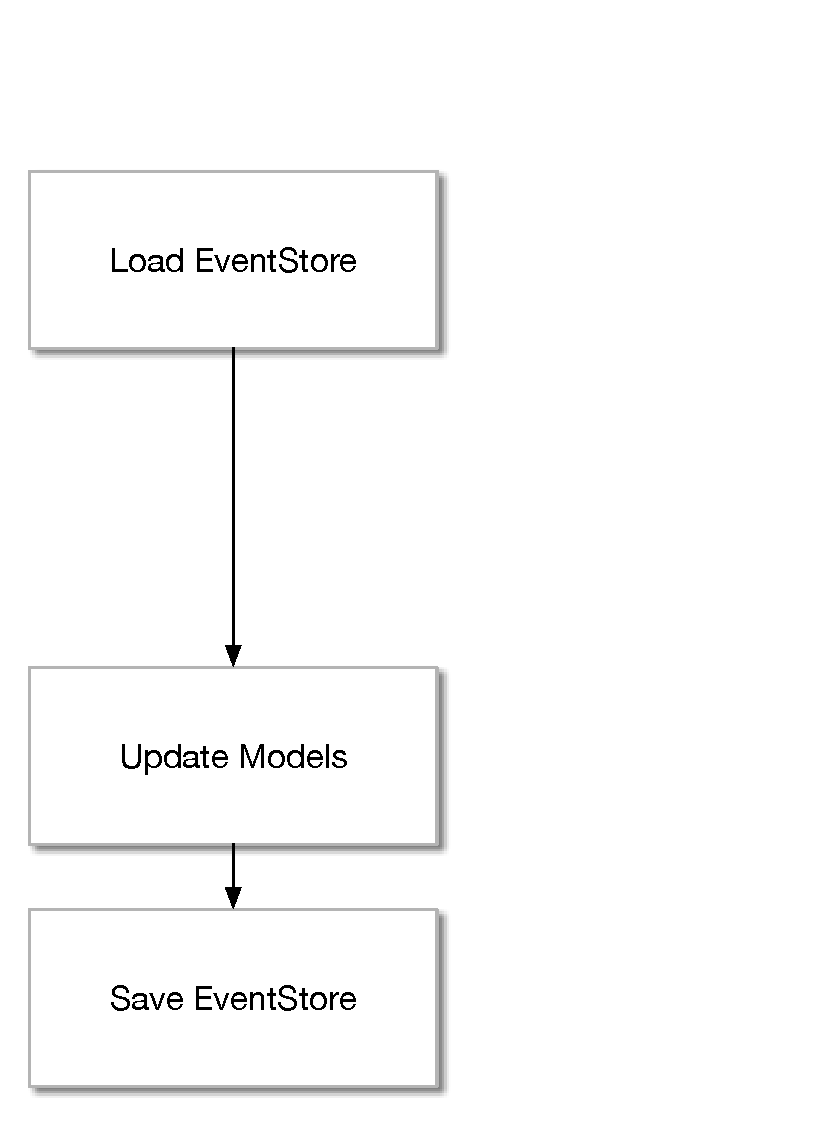
\includegraphics[width=.45\textwidth]{../EliminateWriteConflicts1.pdf}
\end{onlyenv}

\begin{onlyenv}<2>
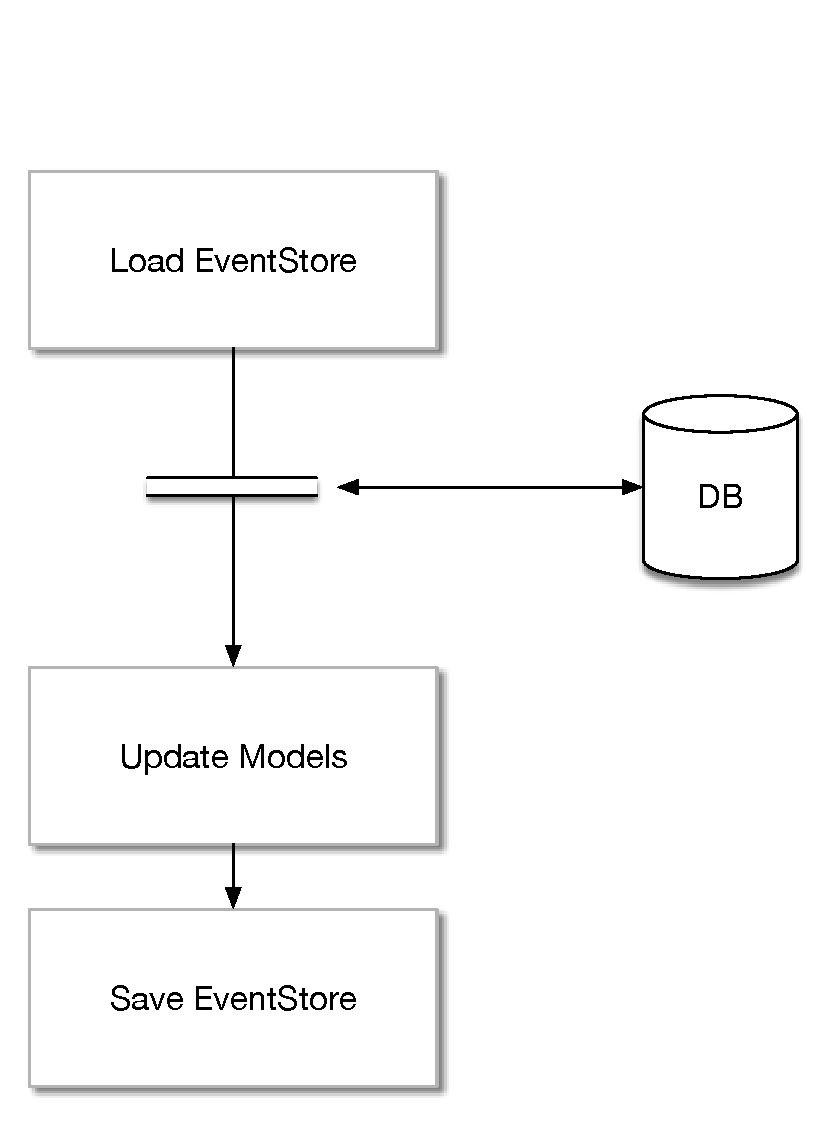
\includegraphics[width=.45\textwidth]{../EliminateWriteConflicts2.pdf}
\end{onlyenv}

\begin{onlyenv}<3>
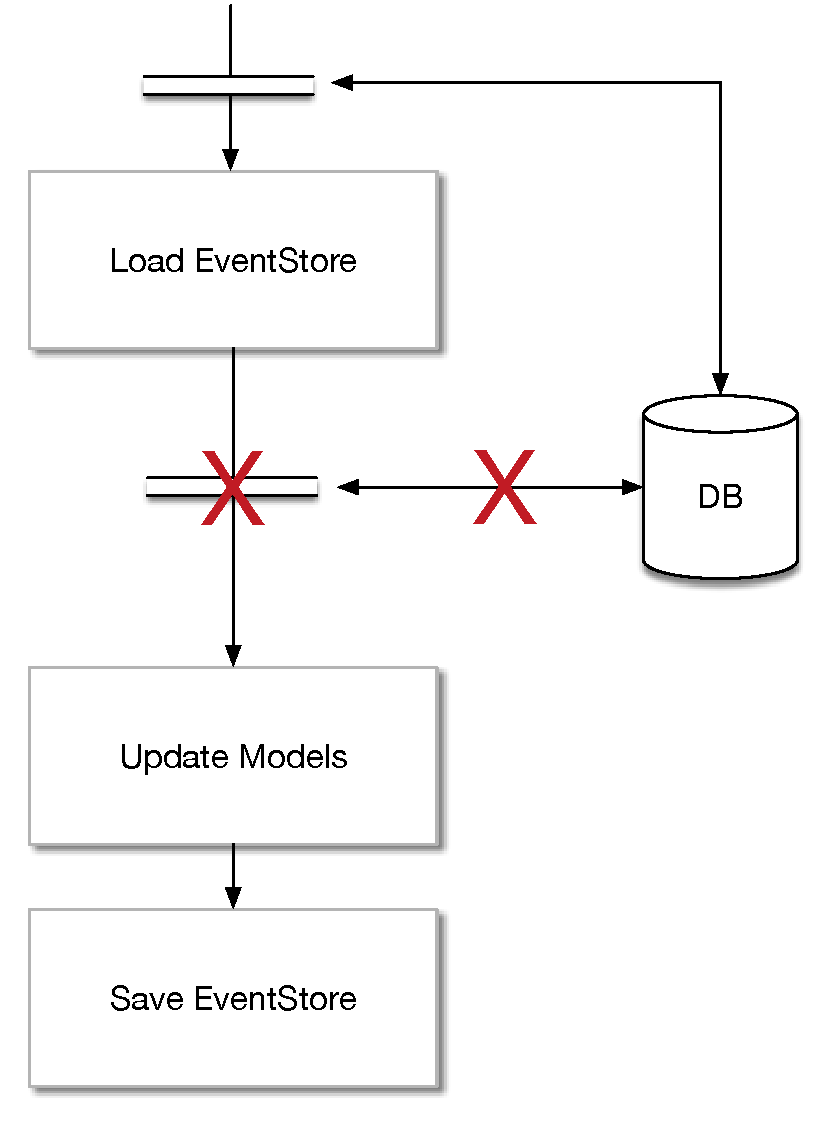
\includegraphics[width=.45\textwidth]{../EliminateWriteConflicts3.pdf}
\end{onlyenv}

\end{center}

\end{frame}


%%%%%%%%%%%%%%%%%%%%%%%%%%%%%%%%%%%%%%%%%%%%%%%%%%
\begin{frame}[fragile]{Benefits}

Synchronous code between loading and updating the event store

\onslide+<2->
\vspace{2em}

$\Longrightarrow$ No possibility for write conflicts

\onslide+<3->
\vspace{2em}

$\Longrightarrow$ We can even save unconditionally

\onslide+<4->
\vspace{2em}

$\Longrightarrow$ Event store is rather a backup

\end{frame}

%%%%%%%%%%%%%%%%%%%%%%%%%%%%%%%%%%%%%%%%%%%%%%%%%%
\begin{frame}[fragile]{Tradeoffs}

We cannot run multiple node.js processes in parallel

\onslide+<2->
\vspace{2em}

$\Longrightarrow$ No way of scaling

\end{frame}

%%%%%%%%%%%%%%%%%%%%%%%%%%%%%%%%%%%%%%%%%%%%%%%%%%
\begin{frame}[fragile]{Takeaways}

\begin{itemize}
\item Event Sourcing: to avoid loss of information
\onslide+<2->
\item Works well in Node.js, if you...
\item ...avoid long load times
\item ...avoid parallelization!
\end{itemize}

\end{frame}


%%%%%%%%%%%%%%%%%%%%%%%%%%%%%%%%%%%%%%%%%%%%%%%%%%
\begin{frame}{Thank you very much!}

        Slides: \url{https://github.com/NicoleRauch/EventSourcingNodeJS} 
        \vspace{1em}

        Code: \url{https://github.com/softwerkskammer/Agora}
        
        ~\\[1em]
        \begin{block}{Nicole Rauch}
        \begin{description}[Twitterxx]
                \item[E-Mail]  \href{mailto:info@nicole-rauch.de}{\texttt{info@nicole-rauch.de}}
                \item[Twitter] \href{http://twitter.com/NicoleRauch}{\texttt{@NicoleRauch}}
                \item[Web] \href{http://www.nicole-rauch.de}{\texttt{http://www.nicole-rauch.de}}
        \end{description}
        \end{block}
\end{frame}


\end{document}

